\chapter{ FEM - Theoretical Foundations and Applications } % Main chapter title

\label{Chapter2 } % For referencing the chapter elsewhere, use \ref{Chapter1} 
% \setlength{\parskip}{0.38cm}

%----------------------------------------------------------------------------------------

\section{Elasticity theory and applications \parencite{ref5}}
Theory of Elasticity presents the theory of stress, deformation and displacement analysis in elastic bodies of different shapes, It is subjected to external causes such as loads, temperature changes, etc. .
%----------------------------------------------------------------------------------------
\section{Solution of the problem of elasticity theory \parencite{ref5} }\label{theory}
In this section, we discuss elastic theoretical equations help to establish the problem.

\begin{itemize}
\item 3 equilibrium equations
    \begin{equation}
        \begin{split}
        \frac{{\partial {\sigma _x}}}{{\partial x}} + \frac{{\partial {\tau _{yx}}}}{{\partial y}} + \frac{{\partial {\tau _{zx}}}}{{\partial z}} + X = 0\\
        \frac{{\partial {\tau _{xy}}}}{{\partial x}} + \frac{{\partial {\sigma _y}}}{{\partial y}} + \frac{{\partial {\tau _{zy}}}}{{\partial z}} + Y = 0\\
        \frac{{\partial {t_{xz}}}}{{\partial x}} + \frac{{\partial {\tau _{yz}}}}{{\partial y}} + \frac{{\partial {\sigma _z}}}{{\partial z}} + Z = 0
        \end{split}
    \end{equation}
\item 6 deformation equations
\begin{list}{+}{}
    \item By Cauchy:
        \begin{equation}
    \begin{split}
        {{\varepsilon _x} = \frac{{\partial u}}{{\partial x}}; \qquad}&{{y_{xy}} = \frac{{\partial u}}{{\partial y}} + \frac{{\partial v}}{{\partial x}}}\\
        {{\varepsilon _y} = \frac{{\partial v}}{{\partial y}}; \qquad}&{{y_{yz}} = \frac{{\partial v}}{{\partial z}} + \frac{{\partial w}}{{\partial y}}}\\
        {{\varepsilon _z} = \frac{{\partial w}}{{\partial z}}; \qquad}&{{y_{zx}} = \frac{{\partial w}}{{\partial x}} + \frac{{\partial u}}{{\partial z}}}
    \end{split}
    \end{equation}
    \item By Saint-Venant:
    \begin{equation}
        \begin{gathered}
\frac{{{\partial ^2}{\gamma _{xy}}}}{{\partial x\partial y}} = \frac{{{\partial ^2}{\varepsilon _x}}}{{\partial {y^2}}} + \frac{{{\partial ^2}{\varepsilon _y}}}{{\partial {x^2}}}\\
\frac{{{\partial ^2}{y_{yz}}}}{{\partial y\partial z}} = \frac{{{\partial ^2}{\varepsilon _y}}}{{\partial {z^2}}} + \frac{{{\partial ^2}{\varepsilon _z}}}{{\partial {y^2}}}\\
\frac{{{\partial ^2}{y_{zx}}}}{{\partial z\partial x}} = \frac{{{\partial ^2}{\varepsilon _z}}}{{\partial {x^2}}} + \frac{{{\partial ^2}{\varepsilon _x}}}{{\partial {z^2}}}\\
2\frac{{{\partial ^2}{\varepsilon _x}}}{{\partial y\partial z}} = \frac{\partial }{{\partial x}}\left( {\frac{{ - \partial {y_{yz}}}}{{\partial x}} + \frac{{\partial {\gamma _{zx}}}}{{\partial y}} + \frac{{\partial {\gamma _{xy}}}}{{\partial z}}} \right)\\
2\frac{{{\partial ^2}{\varepsilon _y}}}{{\partial z\partial x}} = \frac{\partial }{{\partial y}}\left( {\frac{{\partial {y_{yz}}}}{{\partial x}} - \frac{{\partial {y_{zx}}}}{{\partial y}} + \frac{{\partial {y_{xy}}}}{{\partial z}}} \right)\\
2\frac{{{\partial ^2}{\varepsilon _z}}}{{\partial x\partial y}} = \frac{\partial }{{\partial z}}\left( {\frac{{\partial {y_{yz}}}}{{\partial x}} + \frac{{\partial {\gamma _{zx}}}}{{\partial y}} - \frac{{\partial {y_{xy}}}}{{\partial z}}} \right)
\end{gathered}
    \end{equation}
\end{list}
\item Stress-Strain Relationship \parencite{ref4}
\begin{list}{+}{}
\item Stress–strain relationship for isotropic material :

 Robert Hooke was the first one to propose the linear uniaxial stress–strain relation, which states that the stress is proportional to strain. Later, the general relation between the six components of strains and stresses called the generalized Hooke’s law was developed. The generalized Hooke’s law states that each component of stress is a linear combination of strains.

 The stress–strain relationship can be written as: 
 \begin{equation}
    \begin{gathered}
        {\sigma _x} = 2G\left( {{\varepsilon _x} + \frac{{3\mu }}{{1 - 2\mu }}{\varepsilon _{tb}}} \right)\\
        {\sigma _y} = 2G\left( {{\varepsilon _y} + \frac{{3\mu }}{{1 - 2\mu }}{\varepsilon _{tb}}} \right)\\
        {\sigma _z} = 2G\left( {{\varepsilon _z} + \frac{{3\mu }}{{1 - 2\mu }}{\varepsilon _{tb}}} \right)\\
        {\tau _{xv}} = G{Y_{xv}},{\tau _{vz}} = G{Y_{vz}},{\tau _{zx}} = G{Y_{zx}}
\end{gathered}
 \end{equation}

Or we can write it another way:
\begin{equation}
\begin{gathered}
{\varepsilon _x} = \frac{1}{E}\left[ {{\sigma _x} - \mu \left( {{\sigma _y} + {\sigma _z}} \right)} \right]\\
{\varepsilon _y} = \frac{1}{E}\left[ {{\sigma _y} - \mu \left( {{\sigma _x} + {\sigma _z}} \right)} \right]\\
{\varepsilon _z} = \frac{1}{E}\left[ {{\sigma _z} - \mu \left( {{\sigma _x} + {\sigma _y}} \right)} \right]\\
{Y_{xy}} = \frac{{{\tau _{xy}}}}{G};{y_{yz}} = \frac{{{\tau _{yz}}}}{G};{y_{zx}} = \frac{{{\tau _{zx}}}}{G}
\end{gathered}
\end{equation}

\item Stress–strain relationship for Material Nonlinearity:

In non-linear materials, their relationship is non-linear, which we will discuss in the next chapter
\begin{figure}[H]
    \centering
    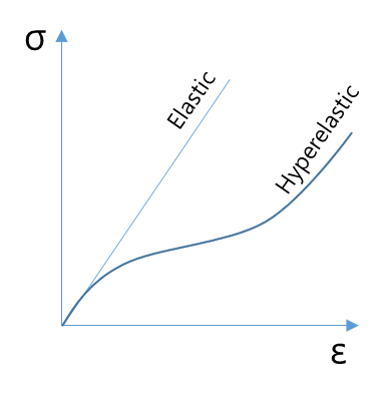
\includegraphics[scale=1]{Figures/Hyperelastic.png}
    \decoRule   
    \caption{ Difference between linear and non-linear material in stress–strain relationship}
    \label{fig:Electron}
\end{figure}
\end{list}
\end{itemize}
%------------------------------------------------------------------------------------------------
%-----------
\section{Finite Element Method (FEM) \parencite{ref4}}
In general, it is difficult to find an analytic solution that satisfies the variational
equation in the previous section. Instead, the FEM divides the entire domain into a
set of simple sub-domains or finite elements. The finite elements are connected with
adjacent elements by sharing their nodes. Then within each finite element, the
solution is approximated in a simple polynomial form.
\vspace{0.38cm}
\newline
FEMs for structural analysis require knowledge of the behavior of each element
in the structure. In this section, a structural analysis based on the finite element
approach is introduced using three-dimensional solid elements. Finite element for-
mulations for other structural elements, such as bars, beams, and plates, etc . Apart from the moreintricate algebra that is required for more complex elements, the basic approach for
deriving element equations is identical to the process illustrated in this section.
Once each element is described, the governing equations of the entire structure may
then be derived.

%------------------------------------------------------------------------------------------------
\section{Finite Element Approximation \parencite{ref4}}
Differential equations and variational equations, introduced in (\ref{theory}) page \pageref{theory},
are difficult to solve, except for a handful of simple cases. When the geometry is
complicated, it is not trivial to solve for u(x) analytically. Since the solution that
satisfies the differential equation and boundary conditions can have a complicated
expression, an infinite series solution may need to be employed. In the FEM, instead
of solving the variational equation analytically, an approximate solution is sought.
The approximate solution u(x) is expressed as a sum of a number of functions that
are called trial functions:
\begin{equation}
\label{eqn:1}
u(x) = \sum\limits_{i = 1}^n {{c_i}} {\phi _i}(x){\rm{ }}
\end{equation}
where $n$ is the number of terms used, $\phi_i(x)$ are known trial functions, and $c_i$ are
coefficients to be determined by minimizing error between the true and the approxi-
mate solution. Since the approximate solution is a linear combination of the trial
functions, the accuracy of approximation depends on them.
\vspace{0.38cm}
\newline
The trial functions and coefficients are chosen such that $u(x)$ must satisfy the
essential boundary conditions of the problem; that is, $u(x)$ must belong to the
space of kinematically admissible displacements, $\mathbb{Z}$. Therefore, if the solution to
the variational equation is approximated by a series of functions in the entire domain
of the problem, it is difficult to obtain the trial functions that satisfy the essential
boundary conditions. An important idea of the FEM is to divide the entire domain
into a set of simple sub-domains or finite elements and then to apply the approximation 
in Eq. (\ref{eqn:1}) on the element level. Then, it is unnecessary to build the trial
functions that satisfy the essential boundary conditions. Instead, only those elements
that include the essential boundary conditions need to have a special treatment.
The finite elements are connected with adjacent elements by sharing their nodes.
Then within each finite element, the solution is approximated using a simple
polynomial form. For example, let us assume that the domain is one-dimensional
and the exact solution is given as a dashed curve in Fig. \ref{fig:Piecewise}. When the entire domain is divided into sub-domains (finite elements), it is possible to approximate the
solution using piecewise continuous linear polynomials as shown in Fig. \ref{fig:Piecewise}.
Within each element, the approximate solution is linear. Two adjacent elements
have the same solution value at the shared node. As can be seen in the figure, when
more numbers of elements are used, the approximate piecewise linear solution will
converge to the exact solution. In addition, the approximation can be more accurate
if higher-order polynomials are used in each element.\\

\begin{figure}[h!]
    \centering
    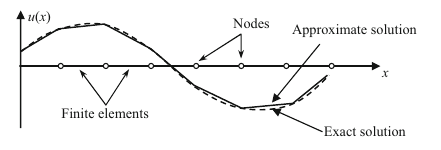
\includegraphics[scale=0.8]{Figures/Chapter2/Piecewise linear approximation.png}
    \decoRule   
    \caption{Piecewise linear approximation of the solution for one-dimensional problem}
    \label{fig:Piecewise}
\end{figure}

%--------------------------------------------------------------
\section{Numerical Integration \parencite{Advance}, \parencite{ref4}}

The integration of the components of the element stiffness matrix, the element mass matrix and
the consistent element load vector was analytically carried out in the previous chapters. In order to have in the development of complex finite elements an adequate tool for the integration of element quantities that are hardly integrable analytically, numerical integration is introduced
and examined for the truss example. By means of numerical integration, it is possible to integrate arbitrary functions in an approximate way. The essential advantages of numerical integration are summarized as follows:
\begin{itemize}
    \item Simplification of the integration
    \item Integration of analytically non-integrable functions
    \item Selective subintegration for elimination of defects from the element formulation
\end{itemize}
In opposition to these advantages there are actually limitations, too:
\begin{itemize}
    \item The generation of element matrices and vectors is numerically costly
     \item The element matrices and vectors are integrated inexactly 3

\end{itemize}

Within the framework of finite element methods, the so-called \textit{Gauss-Legendre Quadrature} has
established itself. The \textsc{Gauss-Legendre} Quadrature of a function $f(\xi 1)$ over the parameter
space $\xi_1 \in [−1, 1]$ is given by the sum
\begin{equation}
\label{eqn:2108}
     \int_{-1}^{1} f\left(\xi_{1}\right) d \xi_{1}=\sum_{i=1}^{n} \alpha^{i} f\left(\xi_{1}^{i}\right) 
\end{equation}
\begin{figure}[H]
    \centering
    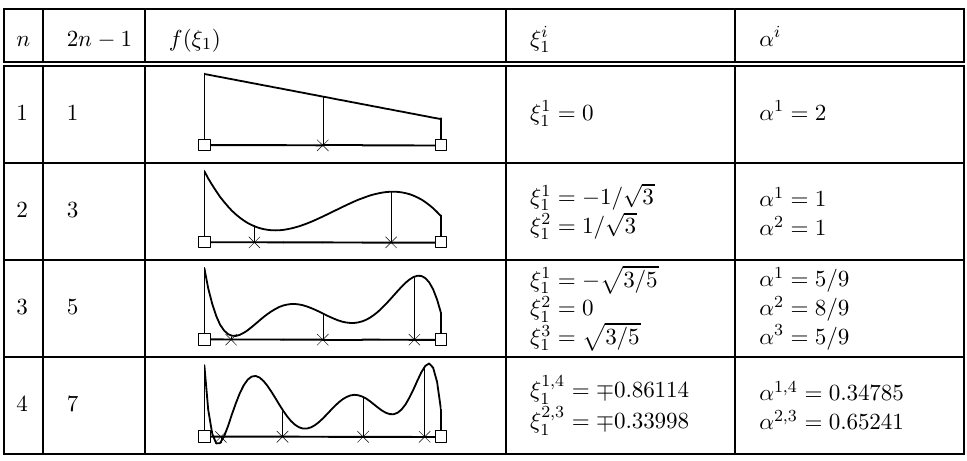
\includegraphics[scale=0.4]{Figures/Chapter2/quadrature.png}
    \caption{\textsc{Gauss} points $\xi_1^i$ and weight factors $\alpha^i$ of the \textsc{Gauss-Legendre} quadrature}
    \label{fig:222}
\end{figure}
In Eq. (\ref{eqn:2108}), $\alpha^i$ are the weight coefficients to the function values $f$ at the supports $\xi_1^i$ and n
is the number of integration points, or so-called \textit{Gauss points}. Polynomials of polynomial degree
\begin{equation}
    p\le 2n-1
\end{equation}
can be integrated exactly by \textsc{Gauss-Legendre} Quadrature, higher-order polynomials and other
functions can be integrated approximately. The linear, quadratic and cubic truss elements are
developed in this section by \textsc{Gauss-Legendre} integration with one and two supports. A summary of $\xi_1^i$ and $\alpha^i$ for $i = 1, 2, 3 $ is found in Figure \ref{fig:222}. For a representation of the fundamentals
of numerical integration, the way of obtaining of the weight factors $alpha^i$ and the \textsc{gauss} points $\xi_1^i$ , refer to the literature of numerical mathematics, e.g. \textsc{Deuflhard & Hohmann}

\textit{\underline{Example: Solve the equation:}}
\begin{equation*}
    x^3+x^2-5x=0
\end{equation*}
Code matlab and result for this problem :
\begin{lstlisting}
syms x;
F=x^3+x^2-5*x;
disp(int(F,[-1 1])); 
%% We take weight Gauss point from quadrature function
[Wgp,Qgp] = quadrature(5,'GAUSS',1); 
f=0;
%% Gauss Quadrature
for i=1 : size(Wgp,1)
    f=f+double(Wgp(i)*subs(F,x,Qgp(i)));
end
disp(f);
\end{lstlisting}

We have result for this example in Matlab : 
\begin{figure}[H]
    \centering
    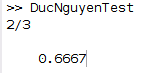
\includegraphics{Figures/Chapter2/resultQuadrature.png}
    \caption{Result for example Quadrature Problem}
    \label{fig:QDTP}
\end{figure}
%---------------------------------------------------------------
\section{Newton Raphson Method \parencite{NewtonRapsonBillboard} \parencite{ref4}}
The \textbf{Newton-Raphson method} (also known as Newton's method) is a way to quickly find a good approximation for the root of a real-valued function $f(x) = 0$ It uses the idea that a continuous and differentiable function can be approximated by a straight line tangent to it.
\subsection{How it Works ?}
Suppose you need to find the root of a continuous, differentiable function f(x)f(x), and you know the root you are looking for is near the point $x = x_0x=x 
0$. Then Newton's method tells us that a better approximation for the root is
\begin{equation}
 x_{1}=x_{0}-\frac{f\left(x_{0}\right)}{f^{\prime}\left(x_{0}\right)} 
\end{equation}
This process may be repeated as many times as necessary to get the desired accuracy. In general, for any $x$-value $x_n$ , the next value is given by
\begin{equation}
 x_{n+1}=x_{n}-\frac{f\left(x_{n}\right)}{f^{\prime}\left(x_{n}\right)} 
\end{equation}
\subsection{Geometric Representation}
Figure \ref{fig:nr1} is the picture to demonstrate what Newton's method actually does:
\begin{figure}[H]
    \centering
    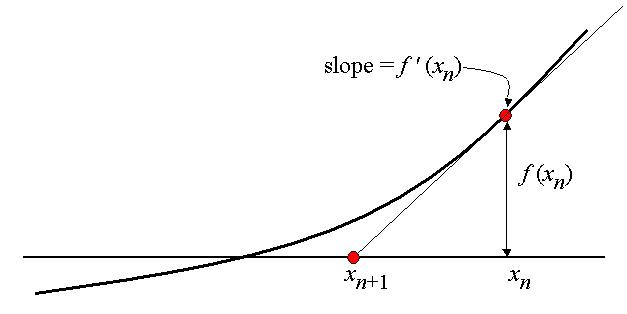
\includegraphics[scale=0.5]{Figures/Chapter2/newtonraphson1.png}
    \caption{Geometric Representation for \textbf{Newton-Raphson} method}
    \label{fig:nr1}
\end{figure}
We draw a tangent line to the graph of $f(x)$ at the point $x = x_n$. This line has slope $f'(x_n) $ and goes through the point $\big(x_n, f(x_n)\big)$
 Therefore it has the equation $y = f'(x_n)(x - x_n) + f(x_n)$. Now, we find the root of this tangent line by setting $y = 0$ and $x=x_{n+1}$ for our new approximation. Solving this equation gives us our new approximation, which is
 $
 x_{n+1}=x_{n}-\frac{f\left(x_{n}\right)}{f^{\prime}\left(x_{n}\right)} 
$
\subsection{Example With Matlab Code}
\label{Example2}
\vspace{0.38cm} \textit{Example: Find the root of the equation $x^2 - 4x - 7 = 0 $ near $x = 5$ to the nearest thousandth.}

We have our $x_0 = 5 $. In order to use Newton's method, we also need to know the derivative of ff. In this case, $f(x) = x^2 - 4x - 7$, and $f'(x) = 2x - 4$

Using Newton's method, we get the following sequence of approximations:
\begin{equation*}
    \begin{gathered}
{x_1} = 5 - \frac{{{5^2} - 4 \times 5 - 7}}{{2 \times 5 - 4}} = 5 - \left( {\frac{{ - 2}}{6}} \right) = \frac{{16}}{3} \approx 5.33333\\
{x_2} = \frac{{16}}{3} - \frac{{{{\left( {\frac{{16}}{3}} \right)}^2} - 4\left( {\frac{{16}}{3}} \right) - 7}}{{2\left( {\frac{{16}}{3}} \right) - 4}} = \frac{{16}}{3} - \frac{{\frac{1}{9}}}{{\frac{{20}}{3}}} = \frac{{16}}{3} - \frac{1}{{60}} = \frac{{319}}{{60}} \approx 5.31667\\
{x_3} = \frac{{319}}{{60}} - \frac{{{{\left( {\frac{{319}}{{60}}} \right)}^2} - 4\left( {\frac{{319}}{{60}}} \right) - 7}}{{2\left( {\frac{{319}}{{60}}} \right) - 4}} = \frac{{319}}{{60}} - \frac{{\frac{1}{{3600}}}}{{\frac{{398}}{{60}}}} \approx 5.31662.\\
{x_4} = 5.31662 - \frac{{{{(5.3362)}^2} - 4(5.3362) - 7}}{{2(5.3362) - 4}} = 5.31662
\end{gathered}
\end{equation*}

Code Matlab base on Newton-Raphson method:
\begin{lstlisting}
function [result,m]=NewtonRaphsonVsCount(x,f,range,n,x0)
%% input la bien so x, ham so f,range, so buoc lap n,x0 (neu co)
%output [result,m,]
%% giai thuat
df=diff(f,x,1);
ddf=diff(f,x,2);
newton= x-f/df;
%% Tim dieu kien bat dau bat fourier 
if exist('x0') == 0
    fourier=double(subs(f*ddf,x,range))
    for i =1:length(range)
        if fourier(i)>=0
            x0=range(i)
        end                             
    end
end
%% tim m de tinh sai so 
m=double(min(subs(abs(df), x, range)));
%% Bat dau giai thuat newton Raphson
X=[x0];
DeltaX=[0];
for i=1:n
    x_n=double(subs(newton,x,X(end)));
    X=[X;x_n];
    DeltaX=[DeltaX ; double(subs(abs(f)/m,x,x_n))];
end
n=[0:n]';
result=table(n,X,DeltaX);

\end{lstlisting}

We build solution for this example base on this function:
\begin{lstlisting}
syms x
range =[4 6];
f=x^2-4*x-7;
x0=5;
n=4;
[result]=NewtonRaphsonVsCount(x,f,range,n,x0);
disp(result)
\end{lstlisting}

\begin{figure}[H]
    \centering
    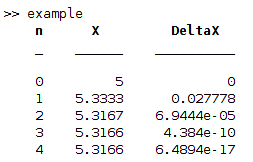
\includegraphics{Figures/Chapter2/resultNewton.png}
    \caption{Result for section \ref{Example2} in Matlab}
    \label{fig:Piecewise}
\end{figure}

\subsection{Limitations of Newton's Method}


Newton's method may not work if there are points of inflection, local maxima or minima around $x_0$  or the root.

For example, suppose you need to find the root of $27x^3 - 3x + 1 = 0$ which is near $x = 0$.
The correct answer is $-0.44157265\ldots$ However, Newton's method will give you the following:

\begin{equation*}
     x_{1}=\frac{1}{3}, x_{2}=\frac{1}{6}, x_{3}=1, x_{4}=0.679, x_{5}=0.463, x_{6}=0.3035, x_{7}=0.114, x_{8}=0.473, \ldots 
\end{equation*}

This is very clearly not helpful. That's because the graph of the function around $x = 0$ looks like in figure \ref{fig:limitNewton}.
\begin{figure}[H]
    \centering
    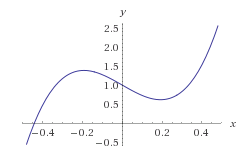
\includegraphics{Figures/Chapter2/limitNewton.png}
    \caption{Example the limit of \textsc{Newton-Raphson} Method }
    \label{fig:limitNewton}
\end{figure}
As you can see, this graph has a local maximum, a local minimum and a point of inflection around $x = 0$. To see why Newton's method isn't helpful here, imagine choosing a point at random between $x = -0.19$ and $x=0.19$ and drawing a tangent line to the function at that point. That tangent line will have a negative slope, and therefore will intersect the $y$-axis at a point that is farther away from the root. So this method doesn't always give the expected result.
\subsection{Significance of Newton-Raphson in Mechanical Solution }
Consider the following system of nonlinear equations:
\begin{equation}
\label{eqn:26}
    P(u)=f
\end{equation}
where $u = [u_1, u_2,\ldots,u^n]^T$ is a vector of unknowns, $f=4 [f_1, f_2,\ldots , f_n]^T$ is a vector of known quantities, and $P(u)= [P_1(u), P_2(u),\ldots, P_n(u)]^T$ is a vector of nonlinear
functions of $u$. In structural applications, $u$ is often the displacement vector, $f$ is the
applied force vector, and $P(u)$ is the internal force vector. Thus, Eq. (\ref{eqn:26}) is the
equilibrium between internal and applied forces. In the linear problems 
the internal force vector is a linear function of u such that $P(u)=K.u$ with $K$ being
a constant stiffness matrix. Then, solving a system of linear equations is equivalent
to calculating the inverse matrix of K and multiplying it with the vector,
$f$. 

Since P(u) is a nonlinear function of $u$, nonlinear analysis focuses on how to solve Eq. (\ref{eqn:26}) accurately and effectively. The solution methods applicable to general nonlinear functions are all iterative. Starting from an initial estimate, $u_0$, the increment, $\Delta u$, of the solution is obtained by solving a system of linear equations. Linearization is involved in this process. After obtaining the increment, the solution is iteratively updated until a specified convergence criterion is satisfied. Different methods are available according to the way to calculate the increment,
$\Delta u$; 

\textsc{Newton-Raphson} method is popular in numerical analysis to find the roots of nonlinear
equations. Basically, most numerical methods for solving a system of nonlinear
equations assume an initial estimate, u0, and find its increment, Δu, so that the
new estimate, $u_0 + \Delta u,$ is close to the solution to Eq. (\ref{eqn:26}). In order to find the increment, the nonlinear equations are locally approximated by linear ones. This process is repeated until the original nonlinear equations are satisfied. these will be discussed in section \ref{sec:nonlinear}.

%---------------------------------------------------------------
\section{Plane Finite Elements \parencite{ref6}}
The Finite Element Method (FEM) is used for finding approximate solutions of partial
differential equations. It is based on an expansion of the dependent variable(s), the
particle flux in our case, into a linear combination of polynomial trial functions defined
over subvolumes. The trial functions space must be chosen so as to ensure that improvement in the numerical approximation occurs with increase in the number I of subvolumes and/or
with the degree K of the polynomial trial functions. The trial functions are known a priori and the corresponding coefficients can be found using a weighted residual approach or a variational formulation. In this section, We have chosen to present the variational formulation, as it brings two important benefits:
\begin{enumerate}
    \item The intrinsic symmetry of the one-speed diffusion equation is always preserved by
the discretization process,
    \item The boundary conditions are introduced in a consistent way.
\end{enumerate} 

\begin{figure}[h!]
    \centering
    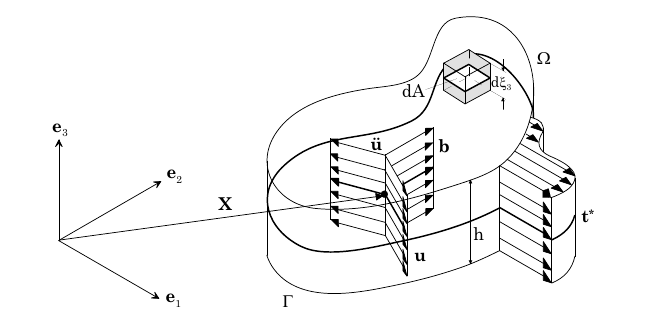
\includegraphics[scale=0.6]{Figures/Chapter2/planeElement.png}
    \decoRule   
    \caption{Representation of the three-dimensional continuum in plane elements}
    \label{fig:plane-element}
\end{figure}
\noindent
The FEM can be applied to various types and form of subvolumes or elements. In the following section first the basic equations of plane finite elements are derived from the
consideration of the three-dimensional continuum with the insertion of the fundamental assumptions of planar continua. Afterwards, plane elements are classified according to the element form and the order of the shape functions and the discretization of planar continua is explained in
details with the help of the four-node, linear, isoparametric Lagrange element. Furthermore,
retangular elements of higher approximation order and are discussed.
%--------
\subsection{Mechanical Problem}
\label{planeproblem}
In this section, we will discuss  two popular problems of the plane element: plane stress and plane strain
\begin{figure}[H]
    \centering
    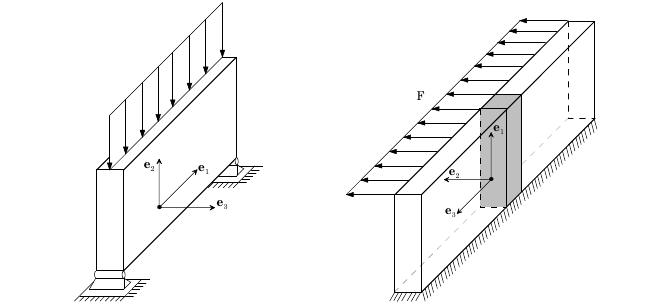
\includegraphics[scale=0.5]{Figures/Chapter2/110.png}
    \decoRule   
    \caption{ Examples for the application of plane stress and strain states}
    \label{fig:110}
\end{figure}
%-----plane strain stress
\vspace{0.38cm} \textbf{a) \textit{Plane Stress State}} \\
A representative plane element is examined, which lies in the plane spanned by the base vectors
$e_1$ and $e_2$ . In the case of a plane stress state it is assumed that the stress components $\sigma_{33}$ , $\sigma_{13}$ and $\sigma_{23}$ vanish

\begin{equation}
\begin{gathered}
  \sigma_{11}=\sigma_{22}=\sigma_{33}=0 \\
    \varepsilon_{13}=\varepsilon_{23}=0
\end{gathered}
\end{equation}
with the remaining stress components being constant in the direction of the base vector $e_3$ , see Fig. \ref{fig:111}
\begin{figure}[H]
    \centering
    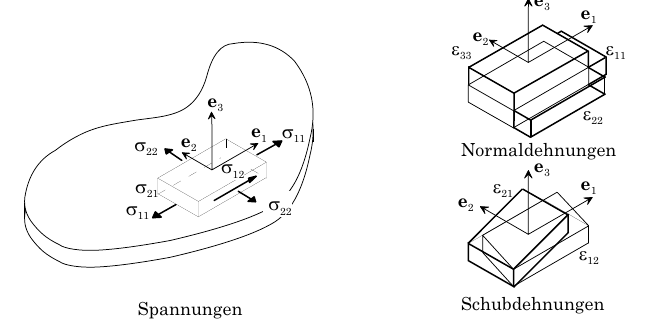
\includegraphics[scale=0.5]{Figures/Chapter2/111.png}
    \decoRule   
    \caption{Plane stress state}
    \label{fig:111}
\end{figure}
%-----plane strain stress
\vspace{0.38cm} \textbf{b) \textit{Plane Strain State}} \\
Again, a representative plane element is examined which lies in the plane spanned by the base
vectors $e_1$ and $e_2$ , see Fig.\ref{fig:112}. For the generation of the plane strain state it is assumed that the strain components $ \varepsilon_{33} , \varepsilon_{13}$ and $\varepsilon_{23} $vanish. the stress components $\sigma_{23} , \sigma_{13}$ become zero; the stress $\sigma_{33}$ , on the contrary, is different from zero.
\begin{equation}
\begin{gathered}
  \varepsilon_{11}=\varepsilon_{22}=\varepsilon_{33}=0 \\
    \sigma_{13}=\sigma_{23}=0
\end{gathered}
\end{equation}
\begin{figure}[H]
    \centering
    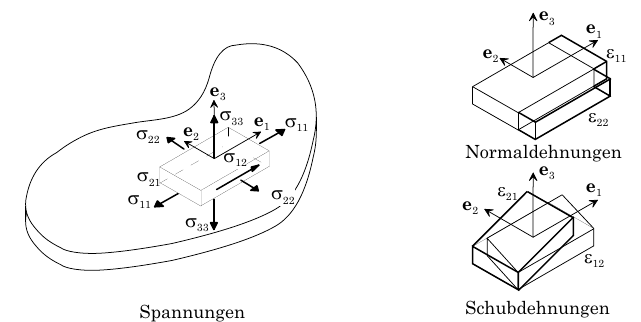
\includegraphics[scale=0.5]{Figures/Chapter2/112.png}
    \decoRule   
    \caption{  Plane strain state}
    \label{fig:112}
\end{figure}
%-------------------------------------------

%-----plane strain stress
\subsection{Geometry}
A planar structure, or a two-dimensional continuum, is generated by the degeneration of the
three-dimensional continuum onto a middle surface A and the thickness h. Due to this reason,
the properties of the three-dimensional continuum are represented by the properties of the
middle surface within the context of the modelling of a plane finite element (see Fig. \ref{fig:plane-element}).
Two-dimensional elements of structural mechanics are
\begin{itemize}
    \item Plane elements which are characterized by a small thickness $h$ relative to the dimensions of the middle surface and are characterized by the plane stress state ( see section \ref{planeproblem})
    
    \item Plane elements which describe an infinite dimension of the mechanical problem in $e _3$ - direction and are, thus, described by the plane strain state ( see section \ref{planeproblem}) 
\end{itemize}
\noindent
The thickness $h$ represents in the case of plane strain state the infinite thickness or the unit
thickness; therefore the thickness of finite elements of the plane strain state is often given the
value one. Within the context of this lecture the element thickness must be considered a parameter also for the plane strain state in order to guarantee a generalized description of elements of
the plane stress and strain state.
The geometrical description of such a two-dimensional element follows from the position vector
of a material point on the middle surface
\begin{equation}
    {\bf X}=[X_1 \quad X_2]^T
\end{equation}
and its motion when a load is applied.

%------------------------------------------------------------------------------------
%------------------------------------------------------------------------------------

\subsection{Kinetics}
The first fundamental assumption for the realization of the degeneration of the three- dimensional continuum to the two-dimensional continuum is the assumption of the stress and strain
state, where it is distinguished between the plane stress state (ES) and the plane strain state
(EV).
\begin{equation}
\label{eqn:3.2}
    \begin{gathered}
ES:{\sigma _{33}} = {\sigma _{23}} = {\sigma _{13}} = 0\\
EV:{\sigma _{33}} = \nu \left( {{\sigma _{11}} + {\sigma _{22}}} \right),{\sigma _{23}} = {\sigma _{13}} = 0
\end{gathered}
\end{equation}
When the plane stress state is assumed to hold the internal kinetics is uniquely described by
the components $\sigma_{11}$ , $\sigma_{22}$ and $\sigma_{12}$ (see Fig.1.11). In the case of plane strain state additionally
the normal stress component $\sigma_{33}$is present (see Fig. 1.12). For a complete and unique
characterization of the stress state this normal component of the stress tensor is actually not
necessary, as it can be computed directly from the stress components $\sigma_{11}$ and $\sigma_{22}$ according to
Eq. (1.74). For the formulation of the internal virtual work the component $\sigma_{33}$ is also of no
significance, for the conjugated strain component $\varepsilon_{33}$ is zero according to the assumptions of
the plane strain state. Therefore, it is enough, both for the plane stress state and for the plane
strain state, to define the stress vector
\begin{equation}
\label{eqn:3.3}
    \sigma=[\sigma_{11} \quad \sigma_{22} \quad \sigma_{33}]^T
\end{equation}

With three components for the formulation of the internal virtual work and, thus, also for the
generation of the discretized stiffness relation of plane finite elements. In accordance woth
the above-mentioned kinetic assumptions the volulme loads $b_3$ and the Neumann boundary
conditions $t^{*}_3$ vanish in the $e_3$-direction, wherefrom also the corresponding vectors are described
by two components each (see Fig. \ref{fig:110}).
\begin{equation}
\label{eqn:3.4}
 \boldsymbol{b}=\left[\begin{array}{ll}b_{1} & b_{2}\end{array}\right]^{T} \qquad \qquad \boldsymbol{t}^{\star}=\left[\begin{array}{ll}t_{1}^{\star} & t_{2}^{\star}\end{array}\right]^{T} 
\end{equation}

%----------------------------------------
\subsection{Kinematics}
The second fundamental assumption of plane finite elements concerns the displacement field:
all material points at the normal of the middle surface exhibit under deformation the same
displacements in the directions $e_1$ and $e_2$ .
\begin{equation}
\label{eqn:3.5}
 u_{1}=u_{1}\left(X_{1}, X_{2}\right) \qquad \qquad u_{2}=u_{2}\left(X_{1}, X_{2}\right) 
 \label{eqn:3.5}
\end{equation}

The displacement component $u_3$ is zero in the case of plane strain state. For the plane stress
state $u_ 3$ is different from zero. However, it follows from the assumptions for the volume and surface loads in Eq. (\ref{eqn:3.4}) that this displacement component has no contribution to the virtual
work of the external loads. Here, it is assumed without a proof 1 that also the portion of this component in the virtual wotk of the inertial forces vanishes during deformation. Thus, the
deformation of the degenerated two-dimensional continuum can be described uniquely by the displacement vector
\begin{equation}
 \boldsymbol{u}\left(X_{1}, X_{2}\right)=\boldsymbol{u}(\boldsymbol{X})=\left[\begin{array}{ll}u_{1}\left(X_{1}, X_{2}\right) & u_{2}\left(X_{1}, X_{2}\right)\end{array}\right]^{T} 
 \label{eqn:3.6}
\end{equation}
expressed, according to Eq. (\ref{eqn:3.5}), only in terms of the coordinates of the plane spanned by the
basis vectors e 1 and e 2 . From this follow directly the variation of the displacement vector and,
by twice differentiating Eq. (\ref{eqn:3.6}) with respect to time, the acceleration vector.
\begin{equation}
\label{eqn:3.7}
 \delta \boldsymbol{u}(\boldsymbol{X})=\left[\delta u_{1}\left(X_{1}, X_{2}\right) \quad \delta u_{2}\left(X_{1}, X_{2}\right)\right]^{T} \qquad \ddot{\boldsymbol{u}}(\boldsymbol{X})=\left[\begin{array}{ll}\ddot{u}_{1}\left(X_{1}, X_{2}\right) & \ddot{u}_{2}\left(X_{1}, X_{2}\right)\end{array}\right]^{T} 
\end{equation}

The complete description of the degenerated two-dimensional continuum requires furthermore the formulation of the Dirichlet boundary conditions
\begin{equation}
\label{eqn:3.8}
 \boldsymbol{u}(\boldsymbol{X}, t)=\boldsymbol{u}^{\star}(\boldsymbol{X}, t\qquad \qquad \forall \quad \boldsymbol{X} \in \Gamma_{u} 
\end{equation}
and the initial conditions of the displacement vector and the acceleration vector, where it should
be noted that only one of the two initial conditions has to be prescribed, as the second one results
from the evaluation of the equation of motion of the degenerated continuum at time $t = 0$
\begin{equation}
\label{eqn:3.9}
 \begin{aligned} \boldsymbol{u}(\boldsymbol{X}, t=0) &=\boldsymbol{u}^{\star}(\boldsymbol{X}) & \qquad \forall \quad \boldsymbol{X} \in \Omega \\ \ddot{\boldsymbol{u}}(\boldsymbol{X}, t=0) &=\ddot{\boldsymbol{u}}^{\star}(\boldsymbol{X}) & & \end{aligned} 
\end{equation}

It remains to describe the strain state of the degenerated continuum by the strain vector $\varepsilon$. In
accordance with the already discussed assumptions of plane stress or plane strain states this
vector can be obtained by the assembly of the strain components$\varepsilon_{ 11 }$, $\varepsilon_ {22}$ and $2\varepsilon_ {12}$ alone.
\begin{equation}
\label{eqn:3.10}
 \varepsilon=\left[\begin{array}{lll}\varepsilon_{11} & \varepsilon_{22} & 2 \varepsilon_{12}\end{array}\right]^{T} 
\end{equation}

The component $\varepsilon_{ 33 }$that is different from zero in the plane stress state is not needed for the unique characterization of the strain state, for this strain component can be combined linearly with the components $\varepsilon_{ 11}$ and $\varepsilon_{ 22}$ . In addition, the same argumentation
for the vanishing virtual work of the strain component $\varepsilon_{ 33}$ as in the definition of the stress vector
$\sigma$, applies here. The strain tensor can be computed in tensor notation
\begin{equation}
\label{eqn:3.11}
 \varepsilon=\nabla^{\mathrm{sym}} \boldsymbol{u} \qquad \qquad \varepsilon_{\alpha \beta}=\frac{1}{2}\left(u_{\alpha, \beta}+u_{\beta, \alpha}\right) 
\end{equation}
where it should be considered that the indices $\alpha$ and $\beta$ can take only the values one or two due to the degeneration ($\alpha$, $\beta$ = 1, 2). Besides, the strain vector can be obtained by application of the differential operator $D_\varepsilon$ to the displacement vector $u$.
\begin{equation}
\label{eqn:3.12}
 \varepsilon=\mathbf{D}_{\varepsilon} u \qquad \qquad
 \left[\begin{array}{c}\varepsilon_{11} \\ \varepsilon_{22} \\ 2 \varepsilon_{12}\end{array}\right]=\left[\begin{array}{cc}\frac{\partial}{\partial X_{1}} & 0 \\ 0 & \frac{\partial}{\partial X_{2}} \\ \frac{\partial}{\partial X_{2}} & \frac{\partial}{\partial X_{1}}\end{array}\right]\left[\begin{array}{l}u_{1} \\ u_{2}\end{array}\right] 
\end{equation}
Thus, it follows directly from the Eqs. (\ref{eqn:3.5}) that the components of the strain vector $\varepsilon_{\alpha \beta}$ are constant along the thickness of the degenerated continuum.

\begin{equation}
\label{eqn:3.13}
 \varepsilon=\varepsilon\left(X_{1}, X_{2}\right) 
\end{equation}
%----------------------------------------
\subsection{Finite Element Discretization}
The finite element discretization and analysis of plane continua consists of the partitioning of
the structure, or the domain under consideration, into finite elements and the approximation
of continuously distributed physical quantities (e.g. displacements) by discrete nodal degrees
of freedom and the assumption of their distribution over the element area. This assumption is
associated with the choice of shape functions, which depend on the variables $\varepsilon_1$ and $\varepsilon_2$ for the case of plane elements.

In contrast to the spatial truss frame, for which a constructively discrete structure was available
already before the mathematical discretization, now a two-dimensional continuum $\Omega$ must be
subdivided into finite subdomains $\Omega^e$ .
\begin{equation}
\label{eqn:3.28}
\begin{gathered}
    \Omega  = \bigcup\limits_{e = 1}^{NE} {{\Omega ^e}}\\
    with \quad {\Omega ^i} \cap {\Omega ^j} = \emptyset {\rm{ }} \quad for \quad i \ne 
\end{gathered}
\end{equation}

Inside these finite subdomains $\Omega^e$ , or finite elements $e$, the continuous field variables are approximated by means of shape functions and discrete nodal degrees of freedom. A basis for the
development of plane finite elements is the requirement that the principle of virtual work should
be fulfilled for every finite element $e$. 
\begin{equation}
\label{eqn:3.29}
 \delta W_{\mathrm{dyn}}^{e}+\delta W_{\mathrm{int}}^{e}=\delta W_{\mathrm{ext}}^{e} 
\end{equation}
The topological element structure, formed by the subdivision into subdomains $\Omega^e$ , is called finite element mesh and the process of its generation is meshing or mesh generation.

Accuracy of the finite element analysis increases with increasing the polynomial degree $p$, for which
reason the basic elements (3- or 4-node elements) are often substituted by elements of higher
polynomial degree. Furthermore, higher-order elements are essentially more suitable than the basic elements for discretizing domains $\Omega$ with curved boundaries, due to the possibility to
describe curved element boundaries. As is to be expected from the previous discussions, \textsc{Lagrange} elements with an internal node provide more accurate results than serendipity elements
without an internal node. The difference in the accuracy is, however, negligible and cannot level
out the shortcoming of the additionally needed internal degrees of freedom of the Lagrange
element (which are of importance particularly by the assembled system). As a disadvantage of
serendipity elements, it should be added that they are restricted to a polynomial degree $p < 4$

\subsection{Shape Functions of Plane Elements }
Within the framework of development of plane finite elements, shape functions of the varying
natural coordinates $\xi_1$ and $ \xi_2$ are used. These shape functions represent polynomials in the
two-dimensional space of the form


\begin{figure}
    \centering
    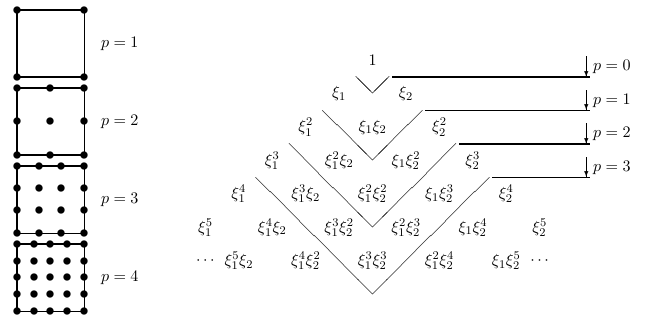
\includegraphics[scale=0.5]{Figures/Chapter2/LagrangePascal.png}
    \caption{Two-dimensional Lagrange ansatz polynomials of quadrangular elements in the
 \textsc{Pascal} triangle  }
    \label{fig:3.5}
\end{figure}


\begin{figure}
    \centering
    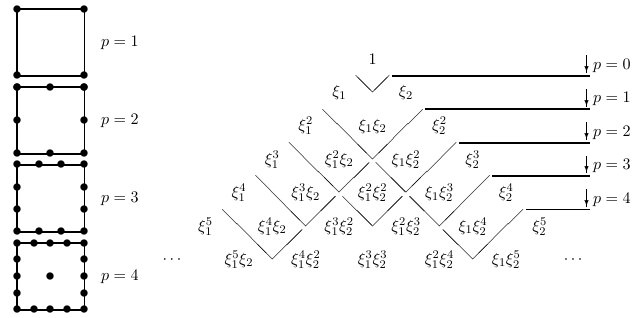
\includegraphics[scale=0.5]{Figures/Chapter2/polynomialsPascal.png}
    \caption{Two-dimensional Serendipity polynomials of quadrangular elements in the \textsc{Pascal}
triangle }
    \label{fig:3.6}
\end{figure}

where the terms of complete two-dimensional polynomials, which correspond to one polynomial
degree and are exempt from the coefficients $\alpha^{ij}$ , can be obtained from the Pascale’s triangle
in Fig. \ref{fig:3.5}. Within the context of development of plane finite elements, the shape functions $N^i (\xi_1 , \xi_2 )$, however, must be generated by multiplication of one-dimensional shape functions or on the basis of interpolation properties. In order to attain
already an idea of the qualitative differences of the finite elements developed in the following
chapters, these elements are characterized by means of the Pascale’s triangle, despite the
planned use of alternative methods for element development.

Complete polynomials of the degree p are derived by multiplication of two one-dimensional
polynomials, also of the degree $p$
\begin{equation}
\label{eqn:3.31}
 \boldsymbol{u}\left(\xi_{1}, \xi_{2}\right) \approx \tilde{\boldsymbol{u}}\left(\xi_{1}, \xi_{2}\right)=\left(\sum_{i=0}^{p} \alpha^{i}\left(\xi_{1}\right)^{i}\right)\left(\sum_{j=0}^{p} \alpha^{j}\left(\xi_{2}\right)^{j}\right) 
\end{equation}

Accordingly, the terms $(\xi_1)^i (\xi_2 )^j$ contained in the Pascale triangle are characterised by the
polynomial degree p of one of the two components paired with all potencies $\le p$ of the other
component. All used terms and thereby developed bilinear, biquadratic, bicubic and biquadratic
Lagrange quadrangular elements are summed up in figure \ref{fig:3.5}. 

\subsection{Serendipity bipolynomials}
Ansatz functions of the Serendipity type are generated with the help of the interpolation feature.
\begin{equation}
    {N^i}\left( {\xi _1^i,\xi _2^i} \right) = 1\qquad {N^i}\left( {\xi _1^j,\xi _2^j} \right) = 0\,\quad {\rm{with }}(i \ne j{\rm{ }})
\end{equation}
The corresponding terms in the Pascal triangle and the resulting finite Serendipity elements are
given in figure \ref{fig:3.6}. Compared to Lagrange ansatz functions, a lesser number of terms is being
used here, due to which a reduced accuracy can be expected compared to the corresponding
Lagrange elements. In order to guarantee at least complete polynomials, Serendipity ansatz
functions have to be furnished with an inner element node as well if the polynomial degree is
greater than $p = 4$, irrespective of the fact that their number is significantly smaller than it is
the case with \textsc{Lagrange} ansatz functions of the same polynomial degree
%---------------------------------------------------------------
\section{Bilinear Lagrange element (Q4) \parencite{LinearStructure}}
The development of plane finite elements is elaborated with the assistance of the relatively simply
generated four-noded bilinear Lagrange element and specified for the case of a rectangular
element.
\subsection{Shape Functions}
The shape function of element node one can be derived by multiplication of the one-dimensional
Lagrange polynomials $N_1^1 (\xi_1 )$ and $N_2^1 (\xi_2 )$ corresponding to this node, which are expressed
in the natural coordinate directions $\xi_1$ or $ \xi_2$ .
\begin{equation}
\label{eqn:3.33}
 N_{1}^{1}\left(\xi_{1}\right)=\frac{1}{2}\left(1-\xi_{1}\right) \quad N_{2}^{1}\left(\xi_{2}\right)=\frac{1}{2}\left(1-\xi_{2}\right) 
\end{equation}
Multiplication of $N_1^1(\xi_1)$ and $N_2^1(\xi_2)$ yields the shape function $N^1(\xi_ 1 , \xi_ 2 )$ for node one. The natural coordinates $\xi_ 1$ and $\xi_ 2$ are assembled in the vector $\xi_ = [\xi_ 1 \xi_ 2 ]$ T in order to show the dependencies.
\begin{equation}
\label{eqn:3.34}
    \label{eqn:334}
    \begin{split}
        {N^1}\left( {{\xi _1},{\xi _2}} \right) &= {N^1}(\xi ) = N_1^1\left( {{\xi _1}} \right)N_2^1\left( {{\xi _2}} \right) \\ &= \frac{1}{2}\left( {1 - {\xi _1}} \right)\frac{1}{2}\left( {1 - {\xi _2}} \right) = \frac{1}{4}\left( {1 - {\xi _1}} \right)\left( {1 - {\xi _2}} \right) \\ &= \frac{1}{4}\left( {1 - {\xi _1} - {\xi _2} + {\xi _1}{\xi _2}} \right)
    \end{split}
\end{equation}
As we can conclude from equation (\ref{eqn:334}), the shape function $N^1(\xi)$ contains constant, linear as
well as bilinear segments. In figure \ref{fig:3.6}, these segments correspond to the square in the Pascal
triangle characterised by $p = 1$. As a preliminary observation to the oncoming explanation of
approximating continuous variables, it may be noted that a two-dimensional polynomial of
plane elements is formed with the sum of all shape functions $N^i(\xi)$ that have the corresponding
weights. The shape functions of the element nodes two to four can be generated in an analogous way.
\begin{equation}
\label{eqn:3.35}
    \begin{gathered}
{N^1}(\xi ) = \frac{1}{4}\left( {1 - {\xi _1}} \right)\left( {1 - {\xi _2}} \right)\\
{N^2}(\xi ) = \frac{1}{4}\left( {1 + {\xi _1}} \right)\left( {1 - {\xi _2}} \right)\\
{N^3}(\xi ) = \frac{1}{4}\left( {1 + {\xi _1}} \right)\left( {1 + {\xi _2}} \right)\\
{N^4}(\xi ) = \frac{1}{4}\left( {1 - {\xi _1}} \right)\left( {1 + {\xi _2}} \right)
\end{gathered}
\end{equation}

Furthermore, in order to approximate the strains and to generate the Jacobi matrix, derivations
of shape functions with respect to the natural coordinates $\xi_ 1$ and $\xi_ 2$ are required. These can
be found as follows:
\[\arraycolsep=10pt\def\arraystretch{3.2}
\begin{equation}
\label{eqn:3.36}
\begin{array}{cccc}
{\dfrac{{\partial {N^1}({\boldsymbol{\xi }})}}{{\partial {\xi _1}}} = N_{;1}^1({\boldsymbol{\xi }}) =  - \dfrac{1}{4}\left( {1 - {\xi _2}} \right)}&{\dfrac{{\partial {N^1}({\boldsymbol{\xi }})}}{{\partial {\xi _2}}} = N_{;2}^1({\boldsymbol{\xi }}) =  - \dfrac{1}{4}\left( {1 - {\xi _1}} \right)}\\
{\dfrac{{\partial {N^2}({\boldsymbol{\xi }})}}{{\partial {\xi _1}}} = N_{;1}^2({\boldsymbol{\xi }}) = \dfrac{1}{4}\left( {1 - {\xi _2}} \right)}&{\dfrac{{\partial {N^2}({\boldsymbol{\xi }})}}{{\partial {\xi _2}}} = N_{;2}^2({\boldsymbol{\xi }}) =  - \dfrac{1}{4}\left( {1 + {\xi _1}} \right)}\\
{\dfrac{{\partial {N^3}({\boldsymbol{\xi }})}}{{\partial {\xi _1}}} = N_{;1}^3({\boldsymbol{\xi }}) = \dfrac{1}{4}\left( {1 + {\xi _2}} \right)}&{\dfrac{{\partial {N^3}({\boldsymbol{\xi }})}}{{\partial {\xi _2}}} = N_{;2}^3({\boldsymbol{\xi }}) = \dfrac{1}{4}\left( {1 + {\xi _1}} \right)}\\
{\dfrac{{\partial {N^4}({\boldsymbol{\xi }})}}{{\partial {\xi _1}}} = N_{;1}^4({\boldsymbol{\xi }}) =  - \dfrac{1}{4}\left( {1 + {\xi _2}} \right)}&{\dfrac{{\partial {N^4}({\boldsymbol{\xi }})}}{{\partial {\xi _2}}} = N_{i2}^4({\boldsymbol{\xi }}) = \dfrac{1}{4}\left( {1 - {\xi _1}} \right)}
\end{array}
\end{equation}
%---------------------------------------------------------
\subsection{Geometry}
The geometry of a four-noded Lagrange element in physical and natural space is shown in figure
\ref{fig:geometry}. An arbitrary material point within the quadrangular element is unequivocally identifiable
by its physical and natural coordinates.
\begin{equation}
 \boldsymbol{X}=\left[\begin{array}{lll}X_{1} & X_{2}\end{array}\right]^{T} \qquad \boldsymbol{\xi}=\left[\begin{array}{ll}\xi_{1} & \xi_{2}\end{array}\right]^{T} 
\end{equation}

Positions of the corner nodes are assembled in the element position vector.
\begin{equation}
    \begin{align}
{X^e} &= {\left[ {\begin{array}{*{20}{c}}
{X_1^{e1}}&{X_2^{e1}}&{X_1^{e2}}&{X_2^{e2}}&{X_1^{e3}}&{X_2^{e3}}&{X_1^{e4}}&{X_2^{e4}}
\end{array}} \right]^T}\\
&= {\left[ {\begin{array}{*{20}{c}}
{{X^e}^{1T}}&{{X^{e2}}^T}&{{X^{e3T}}}&{{X^{e4T}}}
\end{array}} \right]^T}
\end{align}
\end{equation}

Within the scope of isoparametric approximation of geometry and element variables, the continuous position vector $\boldsymbol{X}$ is described with the help of shape functions $N^i(\boldsymbol{\xi})$ in natural coordinates and with the help of discrete positions of element node $\boldsymbol{X}^e}$.

\begin{figure}
    \centering
    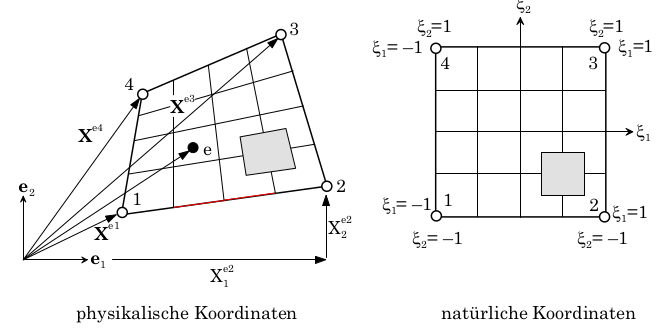
\includegraphics[scale=0.5]{Figure2/Chap2/Bilinear element.png}
    \caption{Bilinear element in physical and natural coordinates}
    \label{fig:geometry}
\end{figure}
\begin{equation}
\label{eqn:339}
 \boldsymbol{X}\left(\xi_{1}, \xi_{2}\right)=\boldsymbol{X}(\boldsymbol{\xi}) \approx \tilde{\boldsymbol{X}}(\boldsymbol{\xi})=\sum_{i=1}^{N \mathrm{~N}} \boldsymbol{X}^{e i} N^{i}(\boldsymbol{\xi})=\sum_{i=1}^{4} \boldsymbol{X}^{e i} N^{i}(\boldsymbol{\xi}) 
\end{equation}
where $NN$ generally stands for the number of element nodes. Alternatively, the continuous
position vector can be approximated by means of the shape function matrix $N(\boldsymbol{\xi})$ and with the
element position vector $\boldsymbol{X}^e$.
\vspace{0.1cm}
\begin{equation}
\small
\underbrace{\left[\begin{array}{c}
\tilde{X}_{1}(\xi) \\
\tilde{X}_{2}(\xi)
\end{array}\right]}_{\bar{X}(\xi)}=\underbrace{\left[\begin{array}{cccccccc}
N^{1}(\xi) & 0 & N^{2}(\xi) & 0 & N^{3}(\xi) & 0 & N^{4}(\xi) & 0 \\
0 & N^{1}(\xi) & 0 & N^{2}(\xi) & 0 & N^{3}(\xi) & 0 & N^{4}(\xi)
\end{array}\right]}_{N(\xi)} \underbrace{\left[\begin{array}{c}
X_{1}^{e 1} \\
X_{2}^{e 1} \\
X_{1}^{e 2} \\
X_{2}^{e 2} \\
X_{1}^{e 3} \\
X_{2}^{e 3} \\
X_{1}^{e 4} \\
X_{2}^{e 4}
\end{array}\right]}_{X^{e}}
\label{eqn:340}
\end{equation}

Equation (\ref{eqn:340}) describes the approximation of physical coordinates as function of natural
coordinates ($NN = 4$)
\begin{equation}
\label{eqn:341}
 \tilde{\boldsymbol{X}}(\boldsymbol{\xi})=\mathbf{N}(\boldsymbol{\xi}) \boldsymbol{X}^{e} \qquad \qquad \boldsymbol{X}^{e}=\left[\begin{array}{lllll}X_{1}^{e 1} & X_{2}^{e 1} & \cdots & X_{1}^{e N N} & X_{2}^{e N N}
\end{array}\right]^{T} 
\end{equation}
by means of shape function matrix $N(\boldsymbol{\xi})$, which is made up of diagonal matrices of shape
functions $N i (\boldsymbol{\xi})$ that correspond to element nodes $i$.
\begin{equation}
\label{eqn:3.42}
 \mathbf{N}^{i}(\boldsymbol{\xi})=\left[\begin{array}{cc}N^{i}(\boldsymbol{\xi}) & 0 \\ 0 & N^{i}(\boldsymbol{\xi})\end{array}\right] \qquad \qquad \mathbf{N}=\left[\begin{array}{lll}\mathbf{N}^{1} & \cdots & \mathbf{N}^{N N}\end{array}\right], NN=4 
\end{equation}

The mapping from natural to physical coordinates according to equations (\ref{eqn:339}) to (\ref{eqn:341}) can be generally described by the functional relation,
\begin{equation}
\label{eqn:3.43}
 \boldsymbol{X}=\boldsymbol{X}(\boldsymbol{\xi}) \qquad \qquad \qquad X_{\beta}=X_{\beta}(\boldsymbol{\xi}), \quad \beta=1,2 
\end{equation}
where the ’Tilda’ approximation designation is omitted. The inverse mapping describes the natural coordinates as function of the physical coordinates.
\begin{equation}
 \boldsymbol{\xi}=\boldsymbol{\xi}(\boldsymbol{X}) \qquad \qquad \qquad \xi_{\alpha}=\xi_{\alpha}(\boldsymbol{X}), \quad \alpha=1,2 
 \label{eqn:3.44}
\end{equation}
\subsection{Jacobi Transformation}
\begin{figure}
    \centering
    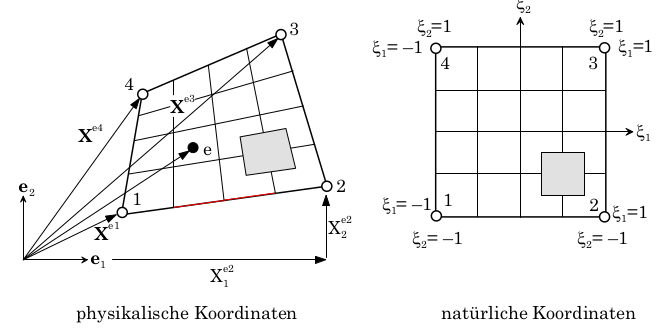
\includegraphics[scale=0.5]{Figure2/Chap2/Bilinear element.png}
    \caption{Jacobi transformation of a surface element $dA$ in natural coordinates}
    \label{fig:3.10}
\end{figure}
The calculation of the strain vector $\varepsilon$ according to equation (\ref{eqn:3.12}) requires that the displacement
components be derivated with respect to physical coordinates X. Since displacement components
as well as approximation of the position vector within the scope of the isoparametric element
concept are expressed as functions of natural coordinates, the necessary derivations with respect
to physical coordinates must be obtained indirectly over the partial derivatives of equation
(\ref{eqn:3.44}). Applying the chain rule to equation (\ref{eqn:3.44}) results in the transformation relation between derivatives with respect to physical and natural coordinates, respectively.
\begin{equation}
\label{eqn:3.45}
 \frac{\partial}{\partial \xi_{\alpha}}=\frac{\partial}{\partial X_{1}} \frac{\partial X_{1}}{\partial \xi_{\alpha}}+\frac{\partial}{\partial X_{2}} \frac{\partial X_{2}}{\partial \xi_{\alpha}}=\frac{\partial}{\partial X_{\beta}} \frac{\partial X_{\beta}}{\partial \xi_{\alpha}} 
\end{equation}

This equation can alternatively be given in the matrix form with the help of the Jacobi matrix $\boldsymbol{J(\xi)}$.
\begin{equation}

 \left[\begin{array}{c}\frac{\partial}{\partial \xi_{1}} \\ \frac{\partial}{\partial \xi_{2}}\end{array}\right]=\left[\begin{array}{ll}\frac{\partial X_{1}}{\partial \xi_{1}} & \frac{\partial X_{2}}{\partial \xi_{1}} \\ \frac{\partial X_{1}}{\partial \xi_{2}} & \frac{\partial X_{2}}{\partial \xi_{2}}\end{array}\right]\left[\begin{array}{c}\frac{\partial}{\partial X_{1}} \\ \frac{\partial}{\partial X_{2}}\end{array}\right] \qquad  \qquad \frac{\partial}{\partial \xi}=\mathbf{J}(\xi) \frac{\partial}{\partial \boldsymbol{X}} 
 \label{eqn:3.46}
\end{equation}

The rule for derivating functions in natural coordinates with respect to physical coordinates is
obtainable by inversion of equation (\ref{eqn:3.46}) with ${\rm{|J(}}\xi {\rm{)|  >  0}}{\rm{.}}$.
\begin{equation}
\label{eqn:3.47}
 \frac{\partial}{\partial \boldsymbol{X}}=\mathbf{J}^{-1}(\boldsymbol{\xi}) \frac{\partial}{\partial \boldsymbol{\xi}} 
\end{equation}
The inverse Jacobi matrix $J_{−1}(\xi)$ needed for this can be obtained directly by inverting the
$2 x 2 $ Jacobi matrix $J(\xi)$
\begin{equation}
\label{eqn:3.48}
 \mathbf{J}^{-1}(\boldsymbol{\xi})=\frac{1}{|\mathbf{J}(\boldsymbol{\xi})|}\left[\begin{array}{cc}\frac{\partial X_{2}}{\partial \xi_{2}} & -\frac{\partial X_{2}}{\partial \xi_{1}} \\ -\frac{\partial X_{1}}{\partial \xi_{2}} & \frac{\partial X_{1}}{\partial \xi_{1}}\end{array}\right] 
\end{equation}
where the Jacobi determinant is given by the expression
\begin{equation}
\label{eqn:3.49}
 |\mathbf{J}|=\frac{\partial X_{1}}{\partial \xi_{1}} \frac{\partial X_{2}}{\partial \xi_{2}}-\frac{\partial X_{1}}{\partial \xi_{2}} \frac{\partial X_{2}}{\partial \xi_{1}} 
\end{equation}
and the derivatives of physical coordinates are obtainable with respect to natural coordinates
from the approximation of the position vector $X = [X_1 X_2 ]^T $according to equations (\ref{eqn:339}) or (\ref{eqn:341}).
\begin{equation}
\label{eqn:3.50}
 \frac{\partial X_{\beta}(\boldsymbol{\xi})}{\partial \xi_{\alpha}}=\sum_{i=1}^{N} X_{\beta}^{e i} N_{; \alpha}^{i}(\boldsymbol{\xi}) \qquad \qquad \frac{\partial \boldsymbol{X}(\boldsymbol{\xi})}{\partial \xi_{\alpha}}=\boldsymbol{X}_{; \alpha}(\boldsymbol{\xi})=\mathbf{N}_{; \alpha}(\boldsymbol{\xi}) \boldsymbol{X}^{e} 
\end{equation}

Formally, we can get the inverse of the Jacobi matrix by applying the chain rule to functional
relation \( X_{\beta}=X_{\beta}(\boldsymbol{\xi}) \) given in equation (\ref{eqn:3.43})
\begin{equation}
\label{eqn:3.51}
 \frac{\partial}{\partial X_{\beta}}=\frac{\partial}{\partial \xi_{1}} \frac{\partial \xi_{1}}{\partial X_{\beta}}+\frac{\partial}{\partial \xi_{2}} \frac{\partial \xi_{2}}{\partial X_{\beta}}=\frac{\partial}{\partial \xi_{\alpha}} \frac{\partial \xi_{\alpha}}{\partial X_{\beta}} 
\end{equation}

Definition of the Jacobi matrix:
\begin{equation}
\label{eqn:3.52}
 \left[\begin{array}{c}\frac{\partial}{\partial X_{1}} \\ \frac{\partial}{\partial X_{2}}\end{array}\right]=\left[\begin{array}{cc}\frac{\partial \xi_{1}}{\partial X_{1}} & \frac{\partial \xi_{2}}{\partial X_{1}} \\ \frac{\partial \xi_{1}}{\partial X_{2}} & \frac{\partial \xi_{2}}{\partial X_{2}}\end{array}\right]\left[\begin{array}{c}\frac{\partial}{\partial \xi_{1}} \\ \frac{\partial}{\partial \xi_{2}}\end{array}\right]
 \qquad \qquad \frac{\partial}{\partial \boldsymbol{X}}=\mathbf{J}^{-1}(\xi) \frac{\partial}{\partial \xi} 
\end{equation}

By means of coefficient comparison of the inverse Jacobi matrix according to equations (\ref{eqn:3.48})
and (\ref{eqn:3.52}), we can get the identities
\begin{equation}
\label{eqn:3.53}
 \begin{aligned} \frac{\partial \xi_{1}}{\partial X_{1}} &=\frac{1}{|\mathbf{J}(\boldsymbol{\xi})|} \frac{\partial X_{2}}{\partial \xi_{2}} & \frac{\partial \xi_{2}}{\partial X_{1}} &=-\frac{1}{|\mathbf{J}(\boldsymbol{\xi})|} \frac{\partial X_{2}}{\partial \xi_{1}} \\ \frac{\partial \xi_{1}}{\partial X_{2}} &=-\frac{1}{|\mathbf{J}(\boldsymbol{\xi})|} \frac{\partial X_{1}}{\partial \xi_{2}} & \frac{\partial \xi_{2}}{\partial X_{2}} &=\frac{1}{|\mathbf{J}(\boldsymbol{\xi})|} \frac{\partial X_{1}}{\partial \xi_{1}} \end{aligned} 
\end{equation}

A transformation relation of the surface element $dA$ can be generated from the first of these
identities in physical and natural coordinates.
\begin{equation}
\label{eqn:3.54}
 d A=d X_{1} d X_{2}=|\mathbf{J}(\boldsymbol{\xi})| d \xi_{1} d \xi_{2} 
\end{equation}
Alternatively, we can derive these transformation relations that are presented in figure 3.10 with
assistance of surface elements, in physical and natural coordinates. For that purpose, vectors
$dX_ 1 , dX_ 2 , d\xi_1 $ and $d\xi$ 2 spanning the surface elements are defined. The surface elements are
given with the help of these definitions by the magnitude of the vector product of vectors $dX_ 1$
and $dX_ 2$ that is $d\xi_1$ and $d\xi_2$ .
\begin{equation}
\label{eqn:3.55}
 \begin{aligned} d A &=\left|d \boldsymbol{X}_{1} \times d \boldsymbol{X}_{2}\right| =\sin \alpha\left|d \boldsymbol{X}_{1}\right|\left|d \boldsymbol{X}_{2}\right| \\
  d A_{\xi} &=\left|d \xi_{1} \times d \boldsymbol{\xi}_{2}\right| =\sin \frac{\pi}{2}\left|d \boldsymbol{\xi}_{1}\right|\left|d \boldsymbol{\xi}_{2}\right| =d \xi_{1} d \xi_{2} \end{aligned} 
  \label{eqn:3.55} 
\end{equation}

Next, vectors $dX_\beta$ are tied with vectors $d\xi_\alpha$  with the help of equation (\ref{eqn:3.45}).
\begin{equation}
\label{eqn:3.56}
 d \boldsymbol{X}_{\beta}=\frac{\partial X_{\beta}}{\partial \xi_{\alpha}} d \boldsymbol{\xi}_{\alpha}=\frac{\partial X_{\beta}}{\partial \xi_{1}} d \boldsymbol{\xi}_{1}+\frac{\partial X_{\beta}}{\partial \xi_{1}} d \boldsymbol{\xi}_{1} 
 \label{eqn:3.56} 
\end{equation}

The square of surface element $dA$ comes as result of a vector scalar product of $d_1 x dX_2$ (see
equation (\ref{eqn:3.55})), where equation (\ref{eqn:3.56}) can be introduced instead of $dX_\beta$ .

\begin{equation}
\label{eqn:3.57}
 \begin{aligned} d A^{2}=&\left(d \boldsymbol{X}_{1} \times d \boldsymbol{X}_{2}\right) \cdot\left(d \boldsymbol{X}_{1} \times d \boldsymbol{X}_{2}\right)=\left(d \boldsymbol{X}_{1} \times d \boldsymbol{X}_{2}\right)^{2} \\=&\left[\left(\frac{\partial X_{1}}{\partial \xi_{1}} d \boldsymbol{\xi}_{1}+\frac{\partial X_{1}}{\partial \xi_{2}} d \boldsymbol{\xi}_{2}\right) \times\left(\frac{\partial X_{2}}{\partial \xi_{1}} d \boldsymbol{\xi}_{1}+\frac{\partial X_{2}}{\partial \xi_{2}} d \boldsymbol{\xi}_{2}\right)\right]^{2} \\=&[\frac{\partial X_{1}}{\partial \xi_{1}} \frac{\partial X_{2}}{\partial \xi_{1}} \underbrace{d \boldsymbol{\xi}_{1} \times d \boldsymbol{\xi}_{1}}_{\mathbf{0}}+\frac{\partial X_{1}}{\partial \xi_{1}} \frac{\partial X_{2}}{\partial \xi_{2}} d \boldsymbol{\xi}_{1} \times d \boldsymbol{\xi}_{2}\\ &+\frac{\partial X_{1}}{\partial \xi_{2}} \frac{\partial X_{2}}{\partial \xi_{1}} \underbrace{d \boldsymbol{\xi}_{2} \times d \boldsymbol{\xi}_{1}}_{-d \boldsymbol{\xi}_{1} \times d \boldsymbol{\xi}_{2}}+\frac{\partial X_{1}}{\partial \xi_{2}} \frac{\partial X_{2}}{\partial \xi_{2}} \underbrace{d \boldsymbol{\xi}_{2} \times d \boldsymbol{\xi}_{2}}_{\mathbf{0}}]^{2} \\=& \underbrace{\left[\frac{\partial X_{1}}{\partial \xi_{1}} \frac{\partial X_{2}}{\partial \xi_{2}}-\frac{\partial X_{1}}{\partial \xi_{2}} \frac{\partial X_{2}}{\partial \xi_{1}}\right]^{2}}_{|\mathbf{J}|^{2}} \underbrace{\left[d \boldsymbol{\xi}_{1} \times d \boldsymbol{\xi}_{2}\right]^{2}}_{d A_{\xi}^{2}}=|\mathbf{J}|^{2} d A_{\xi}^{2}=|\mathbf{J}|^{2} d \xi_{1}^{2} d \xi_{2}^{2} \end{aligned} 
 \label{eqn:3.57} 
\end{equation}

The Jacobi determinant here is identified by comparison to the Jacobi matrix determinant
according to equation (\ref{eqn:3.49}), and the surface element is obtained in natural coordinates by
means of comparison to equation (\ref{eqn:3.5}). The connection between the very surface elements
turns out to be trivial by forming the square root of equation (\ref{eqn:3.57}).
\begin{equation}
\label{eqn:3.58}
 d A=|\mathbf{J}(\boldsymbol{\xi})| d \xi_{1} d \xi_{2} 
\end{equation}

%-----------------------------------------
\subsection{Approximation of Element Quantities}
\begin{figure}[H]
    \centering
    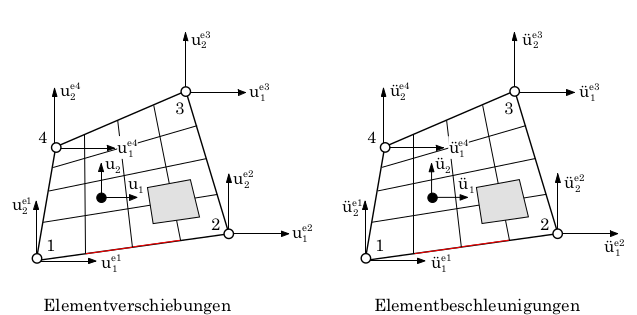
\includegraphics[scale=0.5]{Figure2/Chap2/4nodefredome.png}
    \caption{Degrees of freedom of a four-noded plane Lagrange element}
    \label{fig:3.11}
\end{figure}

Within the scope of the isoparametric element concept we can approximate the continuous
displacements, variation and second time derivative of displacements for $NN = 4$, analogous
with the approximation of the position vector in equation (\ref{eqn:341}) (see figure \ref{fig:3.11}).

\begin{equation}
 \begin{aligned} 
 \boldsymbol{u}(\boldsymbol{\xi}) & \approx \tilde{\boldsymbol{u}}(\boldsymbol{\xi})=\mathbf{N}(\boldsymbol{\xi}) \boldsymbol{u}^{e} & \boldsymbol{u}^{e} &=\left[\begin{array}
 {lllll}u_{1}^{e 1} & u_{2}^{e 1} & \cdots & u_{1}^{e N \mathrm{~N}} & u_{2}^{e N \mathbb{N}}
 \end{array}\right]^{T} \\ 
 \delta \boldsymbol{u}(\boldsymbol{\xi}) & \approx \delta \tilde{\boldsymbol{u}}(\boldsymbol{\xi})=\mathbf{N}(\boldsymbol{\xi}) \delta \boldsymbol{u}^{e} & \delta \boldsymbol{u}^{e} &= \left[
 \begin{array}{lllll}
     \delta u_{1}^{e 1}& \delta u_{2}^{e 1} &\cdots &\delta u_{1}^{e NN} &\delta u_{2}^{e N N}
 \end{array}
\right]^{T}   \\ 
 \ddot{\boldsymbol{u}}(\boldsymbol{\xi}) & \approx \tilde{\tilde{\boldsymbol{u}}}(\boldsymbol{\xi})=\mathbf{N}(\boldsymbol{\xi}) \ddot{\boldsymbol{u}}^{e} & \ddot{\boldsymbol{u}}^{e}
 &=\left[\begin{array}{lllll}\ddot{u}_{1}^{e 1} & \ddot{u}_{2}^{e 1} & \cdots & \ddot{u}_{1}^{e NN} & \ddot{u}_{2}^{e NN}\end{array}\right]^{T} 
 \end{aligned} 
 \label{eqn:3.59} 
\end{equation}

\subsection{Strain vector approximation}
To formulate the internal virtual work, the approximation of which is given with the help of
shape polynomials applied to displacements, and thereupon following integration of stiffness
terms, the strain vector components ought to be described in natural coordinates. This is ac-
complished by applying the derivation rule (\ref{eqn:3.51}) to the displacement strain relation in equation
\begin{equation}
\label{eqn:3.60} 
 \left[\begin{array}{c}\varepsilon_{11} \\ \varepsilon_{22} \\ 2 \varepsilon_{12}\end{array}\right]=\underbrace{\left[\begin{array}{ccc}\frac{\partial \xi_{1}}{\partial X_{1}} \frac{\partial}{\partial \xi_{1}}+\frac{\partial \xi_{2}}{\partial X_{1}} \frac{\partial}{\partial \xi_{2}} & 0 & \\ 0 & \frac{\partial \xi_{1}}{\partial X_{2}} \frac{\partial}{\partial \xi_{1}}+\frac{\partial \xi_{2}}{\partial X_{2}} \frac{\partial}{\partial \xi_{2}} \\ \frac{\partial \xi_{1}}{\partial X_{2}} \frac{\partial}{\partial \xi_{1}}+\frac{\partial \xi_{2}}{\partial X_{2}} \frac{\partial}{\partial \xi_{2}} & \frac{\partial \xi_{1}}{\partial X_{1}} \frac{\partial}{\partial \xi_{1}}+\frac{\partial \xi_{2}}{\partial X_{1}} \frac{\partial}{\partial \xi_{2}}\end{array}\right]}_{\mathbf{D}_{\varepsilon \xi}}\left[\begin{array}{c}u_{1} \\ u_{2}\end{array}\right], \quad \varepsilon=\mathbf{D}_{\varepsilon \xi} u 
\end{equation}

With the approximation of continuous displacements according to equation (\ref{eqn:3.59}), we get the
approximation of the strain vector from equation (\ref{eqn:3.60})
\begin{equation}
 \varepsilon(\boldsymbol{\xi}) \approx \tilde{\varepsilon}(\boldsymbol{\xi})=\mathbf{D}_{\varepsilon \xi}(\boldsymbol{\xi}) \tilde{\boldsymbol{u}}(\boldsymbol{\xi})=\mathbf{D}_{\varepsilon \xi}(\boldsymbol{\xi}) \mathbf{N}(\boldsymbol{\xi}) \boldsymbol{u}^{e}=\mathbf{B}(\boldsymbol{\xi}) \boldsymbol{u}^{e} \label{eqn:3.61} 
\end{equation}
by means of linear mapping of the element displacement vector and the differential operator
definition $\boldsymbol{B(\xi)}$.
\begin{equation}
\label{eqn:3.62}
 \tilde{\varepsilon}(\boldsymbol{\xi})=\mathbf{B}(\boldsymbol{\xi}) \boldsymbol{u}^{e} \qquad \qquad \mathbf{B}(\boldsymbol{\xi})=\mathbf{D}_{\varepsilon \xi}(\boldsymbol{\xi}) \mathbf{N}(\boldsymbol{\xi}) 
\end{equation}

The differential operator $B(\xi)$ is here given by applying $D \varepsilon\xi (\xi)$ to the matrix of shape functions
$N(\xi)$. If the operator $D _{\varepsilon\xi} (\xi)$ is not applied to the entire matrix of shape functions but only to
the submatrices $N i (\xi)$, we obtain the $B$-operator $B i (\xi)$ assigned to the element node i instead
of $B-operator B(\xi)$,
\begin{equation}
 \mathbf{B}_{i}(\boldsymbol{\xi})=\mathbf{D}_{\varepsilon \xi}(\boldsymbol{\xi}) \mathbf{N}^{i}(\boldsymbol{\xi}) \qquad  \qquad \mathbf{B}=\left[\begin{array}{lll}\mathbf{B}_{1} & \cdots & \mathbf{B}_{N \mathbf{N}}\end{array}\right], N N=4 
 \label{eqn:3.63} 
\end{equation}
with the differential operators $B_i(\xi)$ being matrix of the shape functions.
\begin{equation}
 \mathbf{B}_{i}(\boldsymbol{\xi})=\left[\begin{array}{ccc}\frac{\partial \xi_{1}}{\partial X_{1}} \frac{\partial}{\partial \xi_{1}}+\frac{\partial \xi_{2}}{\partial X_{1}} \frac{\partial}{\partial \xi_{2}} & 0 & \\ 0 & & \frac{\partial \xi_{1}}{\partial X_{2}} \frac{\partial}{\partial \xi_{1}}+\frac{\partial \xi_{2}}{\partial X_{2}} & \frac{\partial}{\partial \xi_{2}} \\ \frac{\partial \xi_{1}}{\partial X_{2}} \frac{\partial}{\partial \xi_{1}}+\frac{\partial \xi_{2}}{\partial X_{2}} \frac{\partial}{\partial \xi_{2}} & \frac{\partial \xi_{1}}{\partial X_{1}} \frac{\partial}{\partial \xi_{1}}+\frac{\partial \xi_{2}}{\partial X_{1}} & \frac{\partial}{\partial \xi_{2}}\end{array}\right]\left[\begin{array}{cc}N^{i}(\boldsymbol{\xi}) & 0 \\ 0 & N^{i}(\boldsymbol{\xi})\end{array}\right] 
 \label{eqn:3.64} 
\end{equation}

Finally, by applying the derivation rules we arrive at the portion of B-operator for element
node $i$.
\begin{equation}
 \mathbf{B}_{i}(\boldsymbol{\xi})=\left[\begin{array}{cc}\frac{\partial \xi_{1}}{\partial X_{1}} N_{; 1}^{i}(\boldsymbol{\xi})+\frac{\partial \xi_{2}}{\partial X_{1}} N_{; 2}^{i}(\boldsymbol{\xi}) & 0 \\ 0 & \frac{\partial \xi_{1}}{\partial X_{2}} N_{; 1}^{i}(\boldsymbol{\xi})+\frac{\partial \xi_{2}}{\partial X_{2}} N_{; 2}^{i}(\boldsymbol{\xi}) \\ \frac{\partial \xi_{1}}{\partial X_{2}} N_{; 1}^{i}(\boldsymbol{\xi})+\frac{\partial \xi_{2}}{\partial X_{2}} N_{; 2}^{i}(\boldsymbol{\xi}) & \frac{\partial \xi_{1}}{\partial X_{1}} N_{; 1}^{i}(\boldsymbol{\xi})+\frac{\partial \xi_{2}}{\partial X_{1}} N_{; 2}^{i}(\boldsymbol{\xi})\end{array}\right] 
 \label{eqn:3.65} 
\end{equation}


If the components of the inverse Jacobi matrix $\xi_{\alpha,\beta}$ according to equation (\ref{eqn:3.53}) are replaced by components of the Jacobi matrix $X_{\alpha,\beta}$ , it is possible to write down the $B$-operators $B_i (\xi)$ in the following way:
\begin{equation}
 \mathbf{B}_{i}(\boldsymbol{\xi})=\frac{1}{|\mathbf{J}(\boldsymbol{\xi})|}\left[\begin{array}{cc}\frac{\partial X_{2}}{\partial \xi_{2}} N_{; 1}^{i}(\boldsymbol{\xi})-\frac{\partial X_{2}}{\partial \xi_{1}} N_{; 2}^{i}(\boldsymbol{\xi}) & 0 \\ 0 & -\frac{\partial X_{1}}{\partial \xi_{2}} N_{; 1}^{i}(\boldsymbol{\xi})+\frac{\partial X_{1}}{\partial \xi_{1}} N_{; 2}^{i}(\boldsymbol{\xi}) \\ -\frac{\partial X_{1}}{\partial \xi_{2}} N_{; 1}^{i}(\boldsymbol{\xi})+\frac{\partial X_{1}}{\partial \xi_{1}} N_{; 2}^{i}(\boldsymbol{\xi}) & \frac{\partial X_{2}}{\partial \xi_{2}} N_{; 1}^{i}(\boldsymbol{\xi})-\frac{\partial X_{2}}{\partial \xi_{1}} N_{; 2}^{i}(\boldsymbol{\xi})\end{array}\right] 
 \label{eqn:3.66} 
\end{equation}

Derived in such a way, the B-operators contain matrix terms of the form $X _{\beta,\alpha} $ which again can be described as functions of shape function derivatives $N_{;a}^j(\xi)$ and of element node coordinates $X^{ij}_\beta$ according to equation (\ref{eqn:3.50}).
\begin{equation}
 \frac{\partial X_{\beta}}{\partial \xi_{\alpha}}=\frac{\partial}{\partial \xi_{\alpha}} \sum_{j=1}^{4} X_{\beta}^{e j} N^{j}(\boldsymbol{\xi})=\sum_{j=1}^{4} X_{\beta}^{e j} N_{; \alpha}^{j}(\boldsymbol{\xi}) 
 \label{eqn:3.67} 
\end{equation}
%--------------------------------------------------------------
\subsection{Appproximation of internal virtual work}

The internal virtual work is developed by substituting the stress vector by material law , by modifying the surface element $dA$ and by adjusting the integration
boundaries to natural coordinates $\xi_\alpha \in [{- 1}, 1]$.
\begin{equation}
 \delta W_{\mathrm{int}}^{e}=\int_{-1}^{1} \int_{-1}^{1} \delta \varepsilon(\boldsymbol{\xi}) \cdot \mathbf{C} \varepsilon(\boldsymbol{\xi})|\mathbf{J}(\boldsymbol{\xi})| h d \xi_{1} d \xi_{2} 
 \label{eqn:3.68} 
\end{equation}

Approximation of internal virtual work comes from substitution of the exact strain vector by
the approximated strain vector in equation (\ref{eqn:3.62})
\begin{equation}
 \delta \tilde{W}_{\mathrm{int}}^{e}=\int_{-1-1}^{1} \int_{-1}^{1} \delta \boldsymbol{u}^{e} \cdot \mathbf{B}^{T}(\boldsymbol{\xi}) \mathbf{C} \mathbf{B}(\boldsymbol{\xi}) \boldsymbol{u}^{e}|\mathbf{J}(\boldsymbol{\xi})| h d \xi_{1} d \xi_{2} 
 \label{eqn:3.69} 
\end{equation}

Due to the independence of the natural coordinates $\xi$ of both element displacement vectors $u^e$
and its variation $\epsilon u^e$ , both of these vectors can be exerted from the integral.

\begin{equation}
 \delta \tilde{W}_{\text {int }}^{e}=\delta \boldsymbol{u}^{e} \cdot \int_{-1}^{1} \int_{-1}^{1} \mathbf{B}^{T}(\boldsymbol{\xi}) \mathbf{C} \mathbf{B}(\boldsymbol{\xi})|\mathbf{J}(\boldsymbol{\xi})| h d \xi_{1} d \xi_{2} \boldsymbol{u}^{e}=\delta \boldsymbol{u}^{e} \cdot \mathbf{k}^{e} \boldsymbol{u}^{e} 
\label{eqn:3.70} 
\end{equation}

Here, we have defined the element stiffness matrix of a bilinear plane quadrangular element of
an arbitrary shape.
\begin{equation}
 \mathbf{k}^{e}=\int_{-1}^{1} \int_{-1}^{1} \mathbf{B}^{T}(\boldsymbol{\xi}) \mathbf{C} \mathbf{B}(\boldsymbol{\xi})|\mathbf{J}(\boldsymbol{\xi})| h d \xi_{1} d \xi_{2} 
\label{eqn:3.71} 
\end{equation}

The element thickness can be independent of the location in case of a plane stress state
$(h = h(\xi))$ ; in case of a plane strain state, the element thickness is constant. It is customary to add the integrand which is evaluated and weighed at the Gauss
points and formed with the help of the $B$-operator, the Jacobi determinant and the element
thickness, to the element stiffness matrix. The so called full integration or the $2 x 2$ integration
of a bilinear element accordingly requires four calculations of an integrand and its weighed
addition.
\begin{equation}
 \mathbf{k}^{e} \approx \sum_{i=1}^{2} \sum_{j=1}^{2} \alpha^{i} \alpha^{j} \mathbf{B}^{T}\left(\xi_{1}^{i}, \xi_{2}^{j}\right) \mathbf{C} \mathbf{B}\left(\xi_{1}^{i}, \xi_{2}^{j}\right)\left|\mathbf{J}\left(\xi_{1}^{i}, \xi_{2}^{j}\right)\right| h\left(\xi_{1}^{i}, \xi_{2}^{j}\right) 
 \label{eqn:3.72} 
\end{equation}

Gauss points $\xi_\alpha^i$ and weighting factors $\alpha^i$ of numeric integration can be found in figure \ref{fig:222}. Apart from the full integration, a subintegration of the bilinear element is also introduced with only
one Gauss point in the midpoint of the element. Merely in special cases of element geometry, it
is reasonable to determine the element stiffness by analytical derivation of the $B$-operator and analytical integration. 

\subsection{Approximation of dynamic virtual work}

Besides discretization of internal virtual work, transient mechanical problems also demand discretization of dynamic virtual work. If we, in the principle of virtual displacements, replace the surface element $dA$ and the integration boundaries 
\begin{equation}
 \delta W_{\mathrm{dyn}}^{e}=\int_{-1-1}^{1} \int_{1}^{1} \delta \boldsymbol{u}(\boldsymbol{\xi}) \cdot \ddot{\boldsymbol{u}}(\boldsymbol{\xi})|\mathbf{J}(\boldsymbol{\xi})| \rho h d \xi_{1} d \xi_{2} 
 \label{eqn:3.73} 
\end{equation}
and if we approximate the variation of displacements as well as continuous accelerations with
the assistance of shape functions according to equation (\ref{eqn:3.59}), we get the approximation of
virtual work of inertial forces.
\begin{equation}
 \delta \tilde{W}_{\mathrm{dyn}}^{e}=\delta \boldsymbol{u}^{e} \cdot \int_{-1-1}^{1} \int_{-1}^{1} \mathbf{N}^{T}(\boldsymbol{\xi}) \mathbf{N}(\boldsymbol{\xi})|\mathbf{J}(\boldsymbol{\xi})| \rho h d \xi_{1} d \xi_{2} \ddot{\boldsymbol{u}}^{e}=\delta \boldsymbol{u}^{e} \cdot \mathbf{m}^{e} \ddot{\boldsymbol{u}}^{e} 
 \label{eqn:3.74} 
\end{equation}

For purposes of defining the element mass matrix, we repeatedly took advantage of the fact
that the element vectors $\varepsilon u^e$ and $\ddot{o}^e$ are independent of natural coordinates.
\begin{equation}
 \mathbf{m}^{e}=\int_{-1}^{1} \int_{-1}^{1} \mathbf{N}^{T}(\boldsymbol{\xi}) \mathbf{N}(\boldsymbol{\xi})|\mathbf{J}(\boldsymbol{\xi})| \rho h d \xi_{1} d \xi_{2} 
\label{eqn:3.75} 
\end{equation}
\subsection{Approximation of virtual work of external loads}

The loads acting on a plane element can be divided into loads acting in the field and those acting at the boundaries of the field. Typical loads in the field are gravitational loads whereas actual structural loads are dominated by boundary loads such as pressure.

\vspace{0.38cm} \textbf{a) \textit{Volume loads}} \\

With the help of displacement variation approximation as in equation (\ref{eqn:3.59}), a consistent element load vector of volume loads $b(\xi)$ can be obtained based on external virtual work.
\begin{equation}
 \delta \tilde{W}_{\mathrm{ext}}^{\Omega e}=\delta \boldsymbol{u}^{e} \cdot \int_{-1}^{1} \int_{-1}^{1} \mathbf{N}^{T}(\boldsymbol{\xi}) \boldsymbol{b}(\boldsymbol{\xi})|\mathbf{J}(\boldsymbol{\xi})| \rho h d \xi_{1} d \xi_{2}=\delta \boldsymbol{u}^{e} \cdot \boldsymbol{r}_{p}^{e} 
\label{eqn:3.76} 
\end{equation}

Element vector of volume forces:

\begin{equation}
 \boldsymbol{r}_{p}^{e}=\int_{-1}^{1} \int_{-1}^{1} \mathbf{N}^{T}(\boldsymbol{\xi}) \boldsymbol{b}(\boldsymbol{\xi})|\mathbf{J}(\boldsymbol{\xi})| \rho h d \xi_{1} d \xi_{2} 
 \label{eqn:3.77} 
\end{equation}

Usually, $b$ is not given as dependent of natural coordinates $\xi$ but as function of physical
coordinates X. In such a case, the position of volume load has to be transformed to natural
coordinates $( b(X) \rightarrow b(\xi))$.

\vspace{0.38cm} \textbf{b) \textit{Boundary loads}} \\

The element load vector of element boundary loads $\boldsymbol{t*(\xi)}h$ is derived by observation of external virtual work . Here, the boundary $\Gamma$ σ can here be divided into four
boundaries $\Gamma_i$ i of the element.
\begin{equation}
 \delta W_{\mathrm{ext}}^{\Gamma e}=\int_{\Gamma_{\sigma}} \delta \boldsymbol{u} \cdot \boldsymbol{t}^{\star} h d \Gamma_{\sigma}=\sum_{i=1}^{4} \int_{\Gamma_{i}} \delta \boldsymbol{u} \cdot \boldsymbol{t}^{\star} h d \Gamma_{i}=\sum_{i=1}^{4} \delta W_{\mathrm{ext}}^{\Gamma_{i} e} 
 \label{eqn:3.78} 
\end{equation}

As an example, the proceeding for calculating the consistent equivalent loads is demonstrated
for element boundary three that connects nodes three and four. As shown in figure \ref{eqn:3.12}, the element edge is characterised by the natural coordinate $\xi_2 = 1$.

\begin{equation}
 \delta W_{\mathrm{ext}}^{\Gamma_{3 e}}=\int_{\Gamma_{3}} \delta \boldsymbol{u}\left(\xi_{1}, 1\right) \cdot \boldsymbol{t}^{\star}\left(\xi_{1}, 1\right) h d \Gamma_{3} 
 \label{eqn:3.79} 
\end{equation}

To integrate this integrand over element edge three, the line element $d\gamma_3$ must be transformed
into the natural coordinate $d\xi_1$ . The differential line element here is analysed in physical space. Projection of line element $d\gamma_3$ onto direction $e_1$ yields the differential physical line element $dX_ 1$ , projection onto direction $e_ 2$ yields $dX_2$ . Vice versa, the square of line element can be calculated with the Pythagoras theorem.
\begin{equation}
 d \Gamma_{3}^{2}=d X_{1}^{2}+d X_{2}^{2} 
 \label{eqn:3.80} 
\end{equation}
\begin{figure}
    \centering
    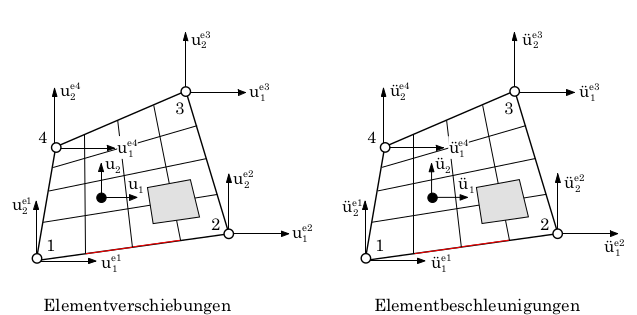
\includegraphics[scale=0.5]{Figure2/Chap2/4nodefredome.png}
    \caption{External loads of a four-noded Lagrange element}
    \label{fig:my_label}
\end{figure}

The total differentials $dX_\beta$ for $ \beta = 1, 2$ are found to be functions of total differentials in natural
coordinates and in Jacobi matrix components. It should be noted here that the differential $d\xi_2$
vanishes $(d\xi _2 = 0) $ at element edge three$ (\xi_ 2 = 1)$.
\begin{equation}
 d X_{\beta}=\frac{\partial X_{\beta}}{\partial \xi_{1}} d \xi_{1}+\frac{\partial X_{\beta}}{\partial \xi_{2}} d \xi_{2}=\frac{\partial X_{\beta}}{\partial \xi_{1}} d \xi_{1} 
\label{eqn:3.81}
\end{equation}

Inserting equation (\ref{eqn:3.81}) into equation (\ref{eqn:3.80}) yields the transformation relation of line element
$d\Gamma_3$ .

\begin{equation}
 d \Gamma_{3}^{2}=\left[\left(\frac{\partial X_{1}}{\partial \xi_{1}}\right)^{2}+\left(\frac{\partial X_{2}}{\partial \xi_{1}}\right)^{2}\right] d \xi_{1}^{2} 
 \label{eqn:3.82} 
\end{equation}

If we additionally introduce the Jacobi determinant$|J_3 (\xi_ 1 , 1)|$, which generally is a function of coordinate $\xi_1$ , we can write down the transformation relation (\ref{eqn:3.82}) in a familiar compact
form.
\begin{equation}
 d \Gamma_{3}=\left|\mathbf{J}_{3}\left(\xi_{1}, 1\right)\right| d \xi_{1} \quad\left|\mathbf{J}_{3}\left(\xi_{1}, 1\right)\right|=\left[\left(\frac{\partial X_{1}}{\partial \xi_{1}}\right)^{2}+\left(\frac{\partial X_{2}}{\partial \xi_{1}}\right)^{2}\right]^{\frac{1}{2}} 
 \label{eqn:3.83} 
\end{equation}

Formally, the same transformation relation is found for line element $d\Gamma_ 1$ , where the partial
derivatives in equation (3.81) must be evaluated for natural coordinate $\xi_ 2 = −1$ instead of
$\xi_ 2 = 1$. Analogous observations lead to transformation relation of line elements $d\Gamma_ 2$ and $d\Gamma_ 4$ .
Transformation of the line element $d\Gamma_ 4$ is given which is valid for both line elements.

\begin{equation}
 d \Gamma_{3}=\left|\mathbf{J}_{3}\left(\xi_{1}, 1\right)\right| d \xi_{1} \qquad \left|\mathbf{J}_{3}\left(\xi_{1}, 1\right)\right|=\left[\left(\frac{\partial X_{1}}{\partial \xi_{1}}\right)^{2}+\left(\frac{\partial X_{2}}{\partial \xi_{1}}\right)^{2}\right]^{\frac{1}{2}} 
 \label{eqn:3.84} 
\end{equation}
Back to element edge three and the boundary load of bilinear Lagrange elements. Next, the
position vector on the element edge according to equation (\ref{eqn:339}) is described with the help
of shape functions $N_ i (\xi_ 1 , 1), i = 1, 2, 3, 4 $, as a basis of transformation (\ref{eqn:3.83}). A reduction
of shape functions is not necessary here since the shape functions corresponding to element
nodes one and two vanish at the element edge three ($N_1 (\xi 1 , 1) = N_2 (\xi 1 , 1) = 0$, see equation
(\ref{eqn:3.35}) 
\begin{equation}
 \boldsymbol{X}\left(\xi_{1}, 1\right)=\sum_{i=1}^{4} \boldsymbol{X}^{e i} N^{i}\left(\xi_{1}, 1\right)=\sum_{i=3}^{4} \boldsymbol{X}^{e i} N^{i}\left(\xi_{1}, 1\right) 
 \label{eqn:3.85} 
\end{equation}

Derivative of the position vector with respect to natural coordinate $\xi_1$ is given by
\begin{equation}
 \frac{\partial \boldsymbol{X}\left(\xi_{1}, 1\right)}{\partial \xi_{1}}=\sum_{i=1}^{4} \boldsymbol{X}^{e i} N_{; 1}^{i}\left(\xi_{1}, 1\right)=\mathbf{N}_{; 1}\left(\xi_{1}, 1\right) \boldsymbol{X}^{e} 
 \label{eqn:3.86} 
\end{equation}
and the derivative with respect to $\xi_2$ is zero. Horizontal and vertical components $dX \beta , \beta = 1, 2$
of line element $ d\Gamma _3 $are found by calculation of total differentials according to equation (\ref{eqn:3.36}),
where derivatives of shape functions according to equation (\ref{eqn:3.81}) are directly used for $\xi_2 = 1$.
\begin{equation}
 d X_{\beta}=\frac{\partial X_{\beta}\left(\xi_{1}, 1\right)}{\partial \xi_{1}} d \xi_{1}=\left[X_{\beta}^{e 3} N_{; 1}^{3}\left(\xi_{1}, 1\right)+X_{\beta}^{e 4} N_{; 1}^{4}\left(\xi_{1}, 1\right)\right] d \xi_{1}=\left[X_{\beta}^{e 3} \frac{1}{2}-X_{\beta}^{e 4} \frac{1}{2}\right] d \xi_{1} 
 \label{eqn:3.87} 
\end{equation}

With equation (\ref{eqn:3.83}), the sought Jacobi determinant $|J_3 (\xi_ 1 , 1)|$ of a bilinear Lagrange element
finally follows, related to element edge three.
\begin{equation}
 \begin{aligned}\left|\mathbf{J}_{3}\left(\xi_{1}, 1\right)\right| &=\left[\left(X_{1}^{e 3} \frac{1}{2}-X_{1}^{e 4} \frac{1}{2}\right)^{2}+\left(X_{2}^{e 3} \frac{1}{2}-X_{2}^{e 4} \frac{1}{2}\right)^{2}\right]^{\frac{1}{2}} \\ &=\frac{1}{2}\left[\left(X_{1}^{e 3}-X_{1}^{e 4}\right)^{2}+\left(X_{2}^{e 3}-X_{2}^{e 4}\right)^{2}\right]^{\frac{1}{2}} \end{aligned}
 \label{eqn:3.88} 
\end{equation}

With this we can substitute the line element dΓ 3 in equation (\ref{eqn:3.79}) as well as the integration
boundaries by a differential of the natural coordinate $\xi_1 $ that is by interval boundaries of the
natural coordinate $\xi_1 \in [−1, 1]$.
\begin{equation}
 \delta W_{\mathrm{ext}}^{\Gamma_{3}}=\int_{-1}^{1} \delta \boldsymbol{u}\left(\xi_{1}, 1\right) \cdot \boldsymbol{t}^{\star}\left(\xi_{1}, 1\right) h\left|\mathbf{J}_{3}\left(\xi_{1}, 1\right)\right| d \xi_{1} 
 \label{eqn:3.89} 
\end{equation}

The approximation of displacement variation according to equation (\ref{eqn:3.59})
\begin{equation}
 \delta \tilde{W}_{\mathrm{ext}}^{\Gamma_{3}}=\delta \boldsymbol{u}^{e} \cdot \int_{-1}^{1} \mathbf{N}^{T}\left(\xi_{1}, 1\right) \boldsymbol{t}^{\star}\left(\xi_{1}, 1\right) h\left|\mathbf{J}_{3}\left(\xi_{1}, 1\right)\right| d \xi_{1}=\delta \boldsymbol{u}^{e} \cdot \boldsymbol{r}_{n 3}^{e} 
 \label{eqn:3.90} 
\end{equation}
finally yields the consistent equivalent load of the boundary load $r^e_{n3}$ .
\begin{equation}
 \boldsymbol{r}_{n 3}^{e}=\int_{-1}^{1} \mathbf{N}^{T}\left(\xi_{1}, 1\right) \boldsymbol{t}^{\star}\left(\xi_{1}, 1\right) h\left|\mathbf{J}_{3}\left(\xi_{1}, 1\right)\right| d \xi_{1} 
 \label{eqn:3.91} 
\end{equation}

The summation of all correspondingly calculated equivalent loads $r_{ni}$ for $i = 1, 2, 3, 4$ yields the
consistent equivalent loads of an element.
\begin{equation}
 \delta \tilde{W}_{\mathrm{ext}}^{\Gamma}=\sum_{i=1}^{4} \delta \tilde{W}_{\mathrm{ext}}^{\Gamma_{i}}=\sum_{i=1}^{4} \delta \boldsymbol{u}^{e} \cdot \boldsymbol{r}_{n i}^{e}=\delta \boldsymbol{u}^{e} \cdot \sum_{i=1}^{4} \boldsymbol{r}_{n i}^{e}=\delta \boldsymbol{u}^{e} \cdot \boldsymbol{r}_{n}^{e} 
 \label{eqn:3.92} 
\end{equation}

The integration of consistent equivalent loads according to equation (3.91) is performed mostly
numerically, too. As opposed to integration of $k _e , m_ e $or $r _{ep} $, one-dimensional numerical integration is necessary here. 
It may be noted here that virtual works of boundary loads of adjacent elements cancel each
other out. For this reason, it is sufficient to calculate the virtual works of boundary loads at free
boundaries that are not only element boundaries but also represent system boundaries.
%-------------------------------------------------------
\section{Biquadratic Serendipity Element (Q8) \parencite{LinearStructure}}
The considerable disadvantage of nine-noded biquadratic Lagrange elements compared to
a bilinear element is the increased number of degrees of freedom. Especially both degrees of
freedom of the middle node are increasing the linear equation system of the assembled system
which has to be solved by two equations per discrete Lagrange element. On the other hand, the
same middle node is not necessary for preservation of compatibility with the adjacent element.

This means that the number of degrees of freedom can especially be reduced at system level
by utilization of serendipity elements instead of Lagrange elements. Hence, the motivation for
generation of quadratic serendipity elements with no middle node is given.

In the sections that follow we will discuss shape functions, approximation of geometry and of
the displacement field. Since the development of the differential operator and of element matrices
and vectors has to be accomplished in analogy with the four-noded or nine-noded Lagrange
element, the presentation of this procedure is abandoned.
\begin{figure}[H]
    \centering
    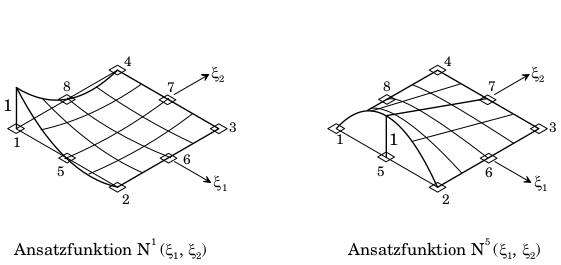
\includegraphics[scale=0.6]{Figure2/Chap2/shpaefunctionq8.png}
    \caption{Generation of biquadratic serendipity shape functions}
    \label{fig:my_label}
\end{figure}

\subsection{Shape Functions}
Contrary to a biquadratic \textsc{Lagrange} element, the shape functions of the eight-noded serendipity element cannot be generated from one-dimensional Lagrange interpolation functions. They
are constructed directly by means of the demands on shape function $N^i(\xi)$ to take on the value
one at node $i$ and the value zero at node $j \ne i$ . The generation of principally different shape functions of corner nodes and side middle nodes is shown in figure {\ref{fig:my_label}.
Here, as an example we have developed the shape functions of corner node one and side middle node eight.

The terms in $\xi_ 1$ and $\xi_ 2 $ appearing in shape functions $ N^ 1 , N^ 5$ and $N^ 8$ are designated by $p = 2$
in the Pascal triangle in figure \ref{fig:3.6}. The remaining shape functions of a quadratic serendipity element are written without deriving.
\begin{equation}
 \begin{aligned} N^{1}(\boldsymbol{\xi}) &=-\frac{1}{4}\left(1-\xi_{1}\right)\left(1-\xi_{2}\right)\left(1+\xi_{1}+\xi_{2}\right) & \qquad N^{5}(\boldsymbol{\xi}) &=\frac{1}{2}\left(1-\xi_{1}^{2}\right)\left(1-\xi_{2}\right) \\ N^{2}(\boldsymbol{\xi}) &=-\frac{1}{4}\left(1+\xi_{1}\right)\left(1-\xi_{2}\right)\left(1-\xi_{1}+\xi_{2}\right) & N^{6}(\boldsymbol{\xi}) &=\frac{1}{2}\left(1+\xi_{1}\right)\left(1-\xi_{2}^{2}\right) \\ N^{3}(\boldsymbol{\xi}) &=-\frac{1}{4}\left(1+\xi_{1}\right)\left(1+\xi_{2}\right)\left(1-\xi_{1}-\xi_{2}\right) & N^{7}(\boldsymbol{\xi}) &=\frac{1}{2}\left(1-\xi_{1}^{2}\right)\left(1+\xi_{2}\right) \\ N^{4}(\boldsymbol{\xi}) &=-\frac{1}{4}\left(1-\xi_{1}\right)\left(1+\xi_{2}\right)\left(1+\xi_{1}-\xi_{2}\right) & N^{8}(\boldsymbol{\xi}) &=\frac{1}{2}\left(1-\xi_{1}\right)\left(1-\xi_{2}^{2}\right) \end{aligned} 
\end{equation}
\subsection{Geometry}
The element coordinate vector X e has a dimension reduced by two as opposed to the vector $X^e$
of a Lagrange element, which corresponds to the coordinates of the middle node.
\begin{equation}
 \boldsymbol{X}^{e}=\left[\begin{array}{llllllll}\boldsymbol{X}^{e 1T} & \boldsymbol{X}^{e 2 T} & \boldsymbol{X}^{e 3 T} & \boldsymbol{X}^{e 4 T} & \boldsymbol{X}^{e 5 T} & \boldsymbol{X}^{\epsilon 6 T} & \boldsymbol{X}^{e 7 T} & \boldsymbol{X}^{e 8 T}\end{array}\right]^{T} 
 \label{eqn:3.151} 
\end{equation}

Geometry of a serendipity element is usually described as function of natural coordinates $\xi$
according to equation (\ref{eqn:3.42}) with the shape functions matrix
\begin{equation}
 \mathbf{N}^{i}(\boldsymbol{\xi})=\left[\begin{array}{cc}N^{i}(\boldsymbol{\xi}) & 0 \\ 0 & N^{i}(\boldsymbol{\xi})\end{array}\right] \quad \mathbf{N}(\boldsymbol{\xi})=\left[\begin{array}{ccccc}\mathbf{N}^{1} & \mathbf{N}^{2} & \cdots & \mathbf{N}^{7} & \mathbf{N}^{8}\end{array}\right] 
 \label{eqn:3.152} 
\end{equation}

%--------------------------------------------
\subsection{Jacobi Transformation}
The \textsc{Jacobi} matrix $J(\xi)$, that is the inverse Jacobi matrix necessary to generate the derivatives with respect to physical coordinates by means of derivatives with respect to natural coordinates,
can be computed in analogy according to equations (\ref{eqn:3.46}) that is (\ref{eqn:3.48}) or
(\ref{eqn:3.52}).
\begin{equation}
 \frac{\partial X_{\beta}(\boldsymbol{\xi})}{\partial \xi_{\alpha}}=\sum_{i=1}^{N N} X_{\beta}^{e i} N_{; \alpha}^{i}(\boldsymbol{\xi}) \qquad \qquad \frac{\partial \boldsymbol{X}(\boldsymbol{\xi})}{\partial \xi_{\alpha}}=\boldsymbol{X}_{; \alpha}(\boldsymbol{\xi})=\mathbf{N}_{; \alpha}(\boldsymbol{\xi}) \boldsymbol{X}^{e} 
 \label{eqn:3.143} 
\end{equation}

Transformation of a differential surface element $dA$ follows according to equation (\ref{eqn:3.58}) with the help of the Jacobi determinant.
%----------------------------------------
\subsection{Approximation of element quantities}

Element quantities, displacements, accelerations and variation of displacements are approxi-
mated in analogy with the Lagrange element.
\begin{equation}
 \begin{aligned} \boldsymbol{u}(\boldsymbol{\xi}) & \approx \tilde{\boldsymbol{u}}(\boldsymbol{\xi})=\mathbf{N}(\boldsymbol{\xi})  \boldsymbol{u}^{e} & \boldsymbol{u}^{e} &=\left[\begin{array}{lllll}u_{1}^{e 1} & u_{2}^{e 1} & \cdots & u_{1}^{e 8} & u_{2}^{e 8}\end{array}\right]^{T} \\ 
 \delta \boldsymbol{u}(\boldsymbol{\xi}) & \approx \delta \tilde{\boldsymbol{u}}(\boldsymbol{\xi})=\mathbf{N}(\boldsymbol{\xi}) \delta \boldsymbol{u}^{e} & \delta \boldsymbol{u}^{e}&=\left[ 
 \begin{array}{lllll}
 \delta u_{1}^{e 1} &\delta u_{2}^{e 1}& \cdots &\delta u_{1}^{e 8}& \delta u_{2}^{e 8}
 \end{array}
 \right]^{T} \\ 
 \ddot{\boldsymbol{u}}(\boldsymbol{\xi}) & \approx \tilde{\tilde{u}}(\boldsymbol{\xi})=\mathbf{N}(\boldsymbol{\xi}) \ddot{u}^{e} & \ddot{\boldsymbol{u}}^{e}&=\left[\begin{array}{lllll}\ddot{u}_{1}^{e 1} & \ddot{u}_{2}^{e 1} & \cdots & \ddot{u}_{1}^{e 8} & \ddot{u}_{2}^{e 8}\end{array}\right]^{T} \end{aligned} 
\end{equation}

The dimension of the element vector is by two smaller than that of an element with a middle
node. Element vectors $u _e$ , $\varepsilon u^e $and $\ddot{u}^ e$ are of dimension $16 × 1$ and the shape function matrix
$\boldsymbol{N}$ is of dimension $2 \times 16$.



% \section{Solution of Non-Linear Static Structural Equations}
% \label{sec:nonlinear}
\vspace{0.38cm}
\newline
With geometrical non-linearity, alterations regarding geometrically linear observation:
\begin{itemize}
    \item Consideration of non-linear terms of the strain tensor E (kinematics)
     \item Establishing the forces equilibrium or application of the impulse theorem in the deformed
configuration (kinetics)

\end{itemize}
We use: 

\begin{itemize}
    \item  (Total) Lagrange point of view which is also described as the material point of view
     \item Stress and strain quantities in the undeformed configuration (second Piola Kirchhoff
stress tensor and Green Lagrange strain tensor)

\end{itemize}



\subsection{Kinematics}
\begin{figure}[h]
    \centering
    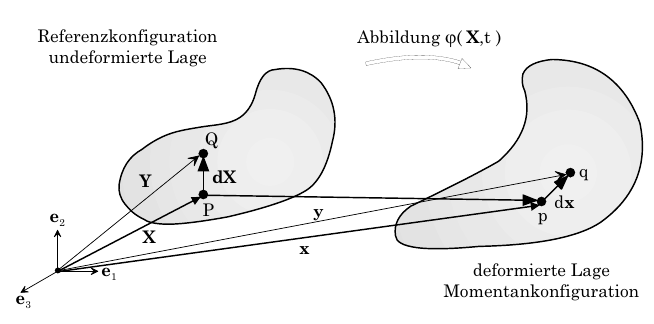
\includegraphics[scale=0.5]{Figures/Chapter2/anh3.png}
    \decoRule   
    \caption{ Current and reference configuration of a deformable material body}
    \label{fig:chap2anh3}
\end{figure}

\noindent
The fundamental of the geometrically non-linear formulation of structural mechanics is based on
the material deformation gradient F , which was already used within the scope of deriving the linear strain tensor  with the help of a non-linear deformation analysis of a material body, and
within the scope of subsequent linearization but not elaborated
because in linear observations it possesses no further significance. Non-linear observations are
a different story where the material deformation gradient defines the transformation from
reference to current configuration or from undeformed to deformed state and vice versa. These
transformations are referred to in technical literature as push forward and pull back. The
material deformation gradient is defined by a transformation of a line element dX of the
reference configuration to the current configuration dx (see figure \ref{fig:chap2anh3} ).

\begin{equation}
    dx = F \cdot dX; \quad F = \frac{{\partial x}}{{\partial X}} = \nabla x
\end{equation}
The Green Lagrange strain tensor E was also already derived and is given in equation (1.12) as function of the displacement gradient $\nabla u$ and its transpose ${\nabla ^T}u$. If we describe the
motion of the material point from the reference to the current configuration with help of the
displacement vector $\bf x = X + u$, the Green Lagrange strain tensor
\begin{equation}
    \label{5.7}
    E = \frac{1}{2}\left[ {{F^T} \cdot F - {\bf{1}}} \right] = {\nabla ^{{\rm{sym}}}}u + \frac{1}{2}{\nabla ^T}u \cdot \nabla u = \frac{1}{2}\left[ {{\nabla ^T}u + \nabla u + {\nabla ^T}u \cdot \nabla u} \right]
\end{equation}
can be represented as a function of the material deformation gradient.
\begin{equation}
 \boldsymbol{F}=\frac{\partial}{\partial \boldsymbol{X}}(\boldsymbol{X}+\boldsymbol{u})=\mathbf{1}+\nabla \boldsymbol{u} 
\end{equation}
According to this relation, the components of the term
\begin{equation}
 \nabla^{\operatorname{sym}} \boldsymbol{u}=\left[\begin{array}{ccc}u_{1,1} & \frac{1}{2}\left(u_{1,2}+u_{2,1}\right) & \frac{1}{2}\left(u_{1,3}+u_{3,1}\right) \\ \frac{1}{2}\left(u_{1,2}+u_{2,1}\right) & u_{2,2} & \frac{1}{2}\left(u_{2,3}+u_{3,2}\right) \\ \frac{1}{2}\left(u_{1,3}+u_{3,1}\right) & \frac{1}{2}\left(u_{2,3}+u_{3,2}\right) & u_{3,3}\end{array}\right] 
\end{equation}
of the linear part of the strain tensor E, given explicitly in equations (1.13) and (1.14), are
supplemented by the term $1/2 \nabla^T u$ · $\nabla u$, in the scope of geometrically non-linear theory, which can again be calculated with the displacement vector gradient according to eq. (1.7)
\begin{equation}
 \nabla \boldsymbol{u}=\left[\begin{array}{lll}u_{1,1} & u_{1,2} & u_{1,3} \\ u_{2,1} & u_{2,2} & u_{2,3} \\ u_{3,1} & u_{3,2} & u_{3,3}\end{array}\right] 
\end{equation}
by matrix multiplication.
\begin{equation}
 \frac{1}{2} \nabla^{T} \boldsymbol{u} \cdot \nabla \boldsymbol{u}=\frac{1}{2}\left[\begin{array}{lll}u_{k, 1}u_{k, 1} & u_{k, 1}u_{k, 2} & u_{k, 1} u_{k, 3} \\ u_{k, 2}u_{k, 1} & u_{k, 2}u_{k, 2} & u_{k, 2}u_{k, 3} \\ u_{k, 3}u_{k, 1} & u_{k, 3}u_{k, 2} & u_{k, 3}u_{k, 3}\end{array}\right] 
\end{equation}
It should be noted that the summation is performed over $k = 1, 2, 3$, respectively. The component presentation of the Green Lagrange strain tensor finally yields the following:
\begin{equation}
\label{5.12}
 E_{i j}=\frac{1}{2}\left(u_{i, j}+u_{j, i}+u_{k, i} u_{k, j}\right); \qquad \boldsymbol{E}=E_{i j} \boldsymbol{E}_{i} \otimes \boldsymbol{E}_{j} 
\end{equation}
In order to formulate the non-linear Finite Element methods, it remains to convert the calculation rule of the strain tensor, given in eq. (\ref{5.7}) or (\ref{5.12}), into the calculation rule of the strain
vector in a suitable way . The linear part of the strain tensor can be expressed as a vector by
application of the differential operator $D_\varepsilon$ to the displacement vector u, as described in eq.
(1.16). However, for the non-linear part of the strain tensor, no suitable operator presentation
can be found.
\begin{equation}
\label{5.13}
    {\bf{E}}({\bf{u}}) = \left[ {\begin{array}{*{20}{c}}
{{E_{11}}}\\
{{E_{22}}}\\
{{E_{33}}}\\
{2{E_{12}}}\\
{2{E_{23}}}\\
{2{E_{13}}}
\end{array}} \right] = \left[ {\begin{array}{*{20}{c}}
{{u_{1,1}}}\\
{{u_{2,2}}}\\
{{u_{3,3}}}\\
{{u_{1,2}} + {u_{2,1}}}\\
{{u_{2,3}} + {u_{3,2}}}\\
{{u_{1,3}} + {u_{3,1}}}
\end{array}} \right] + \left[ {\begin{array}{*{20}{l}}
{1/2\left( {{u_{1,1}}{u_{1,1}} + {u_{2,1}}{u_{2,1}} + {u_{3,1}}{u_{3,1}}} \right)}\\
{1/2\left( {{u_{1,2}}{u_{1,2}} + {u_{2,2}}{u_{2,2}} + {u_{3,2}}{u_{3,2}}} \right)}\\
{1/2\left( {{u_{1,3}}{u_{1,3}} + {u_{2,3}}{u_{2,3}} + {u_{3,3}}{u_{3,3}}} \right)}\\
{{u_{1,1}}{u_{1,2}} + {u_{2,1}}{u_{2,2}} + {u_{3,1}}{u_{3,2}}}\\
{{u_{1,2}}{u_{1,3}} + {u_{2,2}}{u_{2,3}} + {u_{3,2}}{u_{3,3}}}\\
{{u_{1,1}}{u_{1,3}} + {u_{2,1}}{u_{2,3}} + {u_{3,1}}{u_{3,3}}}
\end{array}} \right]{\rm{ }}
\end{equation}
According to eq (\ref{5.13}), the Green Lagrange strain tensor of geometrically non-linear
deformations is obtained by addition of the well-known linear part ${\bf D}_\varepsilon \bf u$ and the non-linear part $\bf E^\textnormal{nl}(u)$,
\begin{equation}
 \boldsymbol{E}(\boldsymbol{u})=\mathbf{D}_{\varepsilon} \boldsymbol{u}+\boldsymbol{E}^{n l}(\boldsymbol{u}) 
\end{equation}
where  ${\bf D}_\varepsilon \bf u$ and $\bf E^\textnormal{nl}(u)$ are defined as follows (summation over $k = 1, 2, 3$).

\begin{equation}
    {{\bf{D}}_\varepsilon }{\bf{u}} = \left[ {\begin{array}{*{20}{c}}
{{u_{1,1}}}\\
{{u_{2,2}}}\\
{{u_{3,3}}}\\
{{u_{1,2}} + {u_{2,1}}}\\
{{u_{2,3}} + {u_{3,2}}}\\
{{u_{1,3}} + {u_{3,1}}}
\end{array}} \right]\qquad {{\bf{E}}^{nl}}({\bf{u}}) = \left[ {\begin{array}{*{20}{l}}
{1/2}{{u_{k,1}}}{{u_{k,1}}}\\
{1/2}{{u_{k,2}}}{{u_{k,2}}}\\
{1/2}{{u_{k,3}}}{{u_{k,3}}}\\
{{u_{k,1}}}{{u_{k,2}}}{}\\
{{u_{k,2}}}{{u_{k,3}}}{}\\
{{u_{k,1}}}{{u_{k,3}}}{}
\end{array}} \right]
\end{equation}



